\documentclass[xcolor=table,aspectratio=169]{beamer}
\usetheme{Madrid}
\usepackage{adjustbox}
\usepackage{dcolumn}
\newcolumntype{d}[1]{D{.}{.}{#1}}
\usepackage[style=verbose-note, sorting=none, sortcites=true, maxnames=1, giveninits=true, autocite=superscript, doi=false, url=false, isbn=false, backend=biber, citetracker=false, pagetracker=false, bibencoding=utf8, eprint=false]{biblatex}
% \usepackage[backend=bibtex,style=authoryear-comp,citestyle=authoryear-comp,firstinits=true,sorting=none,maxnames=1,doi=false,isbn=false,url=false,eprint=false]{biblatex}
\usepackage[T1]{fontenc}

\definecolor{twitter_blue}{HTML}{1da1f2}
\input{seaborn_colours.tex}

% Gobbling first names

\AtEveryCitekey{%
   \clearfield{shorttitle}%
   \clearfield{month}%
   \ifentrytype{article}{%
      \clearfield{title}%
   }{}
   }
\ExecuteBibliographyOptions[online]{eprint=true}

% "blindfootcite" is the equivalent of "footcite" except the number marker does not appear
\newcommand\blfootcite[1]{%
  \begingroup
  \renewcommand\thefootnote{}\footnote{\hspace{-4ex}\cite{#1}}%
  \addtocounter{footnote}{-1}%
  \endgroup
}
\renewcommand*{\multicitedelim}{\textcolor{seaborn_bg_grey_darker}{\addsemicolon}}
\setbeamerfont{footnote}{size=\scriptsize}
\renewcommand\footnoterule{\kern-3pt \color{seaborn_bg_grey_darker}\hrule width \textwidth height 0.4pt \color{black} \kern 2.6pt}

\DeclareSourcemap{
  \maps[datatype=bibtex,overwrite=False]{
   \map{
     \step[fieldsource=journal,
           match={Journal of Chemical Theory and Computation},
           replace={JCTC}]
     \step[fieldsource=journal,
           match={Reviews of Modern Physics},
           replace={Rev. Mod. Phys.}]
     \step[fieldsource=journal,
           match={Reports on Progress in Physics},
           replace={Rep. Prog. Phys.}]
     \step[fieldsource=journal,
           match={Physical Review Letters},
           replace={Phys. Rev. Lett.}]
     \step[fieldsource=journal,
           match={Physical Review},
           replace={Phys. Rev.}]
     \step[fieldsource=journal,
           match={B - Condensed Matter and Materials Physics},
           replace={B}]
     \step[fieldsource=journal,
           match={Journal of Chemical Physics},
           replace={J. Chem. Phys.}]
     \step[fieldsource=journal,
           match={Annual Review of Materials Research},
           replace={Annu. Rev. Mater. Res.}]
   }
  }
}

\renewbibmacro{in:}{}
\DeclareFieldFormat{pages}{\mkfirstpage{#1}}
\beamertemplatenavigationsymbolsempty
\bibliography{references.bib}
\setbeamertemplate{bibliography item}[text]
\renewbibmacro{in:}{}
\AtEveryBibitem{\clearfield{title}}
\AtEveryBibitem{\clearfield{month}}
\AtEveryBibitem{\clearfield{pages}}
\AtEveryBibitem{\clearfield{note}}
\DeclareNameAlias{default}{given-family}

% \renewcommand*{\bibfont}{\tiny}
\usepackage{amssymb}
\usepackage{epsfig}
\usepackage{psfrag}
\usepackage{wrapfig}
\usepackage{graphicx}
\usepackage{color}
\usepackage[table]{xcolor}
\usepackage{amsmath}
\usepackage{multimedia}
\usepackage{subcaption}
%\usepackage{style}
\usepackage{verbatim}
\usepackage{multicol}
\usepackage[table]{xcolor}
\usepackage{tabularx}
% Tikz
\usepackage{tikz}
\usetikzlibrary{positioning,shapes,arrows,backgrounds,fit,calc,external,trees,tikzmark}
% \tikzexternalize[prefix=tikzfigures/]
\tikzstyle{dummy} = []
\tikzstyle{line} = [draw, thick, -latex']
\tikzstyle{headless_line} = [draw, thick, -]
\tikzstyle{default}    = [rectangle, text centered, rounded corners, text=black, font=\sffamily\footnotesize, align=center]
\tikzstyle{default_text}    = [rectangle, text width=10cm, text=black,anchor=north west, font=\sffamily]
\tikzstyle{boxwhite} = [default, fill=white, rounded corners=0.1cm]
\tikzstyle{cp}    = [default, fill=seaborn_blue, text=white, text width=2.8cm, minimum height=0.7cm]
\tikzstyle{pw}    = [cp, fill=seaborn_green]
\tikzstyle{wannier90}    = [cp, fill=seaborn_cyan]
\tikzstyle{bespoke}    = [cp, fill=seaborn_magenta]
\tikzstyle{kcw}    = [cp, fill=seaborn_yellow]
\tikzstyle{w2k}    = [cp, fill=seaborn_magenta]
\tikzstyle{observable}    = [cp, fill=seaborn_red]
\tikzstyle{label} = [circle, text=white, fill=black, font=\sffamily\tiny\bfseries, minimum size=0.3cm, inner sep=1pt]
\tikzset{
  -|-/.style={
    to path={
      (\tikztostart) -| ($(\tikztostart)!#1!(\tikztotarget)$) |- (\tikztotarget)
      \tikztonodes
    }
  },
  -|-/.default=0.5,
  |-|/.style={
    to path={
      (\tikztostart) |- ($(\tikztostart)!#1!(\tikztotarget)$) -| (\tikztotarget)
      \tikztonodes
    }
  },
  |-|/.default=0.5,
}

\newlength{\myyshift}
\setlength{\myyshift}{0.05cm}

\usepackage{lipsum}
\usetikzlibrary{calc}
\newlength{\myfigscale}
\setlength{\myfigscale}{0.3cm}
\usepackage{smartdiagram}
\usesmartdiagramlibrary{additions}
\usepackage{multicol}
\usepackage{helvet}
% \usepackage{sansmath}
% \sansmath
\usepackage{cancel} % for \cancel
\usepackage[normalem]{ulem} % for sout (strike out)
\usepackage{tcolorbox}
\tcbuselibrary{skins,hooks}
\tcbset{colframe=structure,fonttitle=\bfseries,beamer, clip upper, boxsep=0pt, sharp corners=all, no shadow, left skip=0pt, right skip=0pt, coltext=white}

% For electron orbital diagrams
\usepackage{tikzorbital}
% Changing defaults
\pgfkeys{tikzorbital/drawLevel/width = 0.666666}
\pgfkeys{tikzorbital/drawLevel/style = {line width = 1pt, color = black!80, line cap = round}}
\pgfkeys{tikzorbital/drawLevel/spinlength = 0.666666}
\pgfkeys{tikzorbital/drawLevel/spinstyle = {very thick, color = black!80, -stealth}}

\input{seaborn_colours.tex}

% For tikz diagrams with nodes appearing on each slide
\tikzset{
  invisible/.style={opacity=0},
  visible on/.style={alt={#1{}{invisible}}},
  alt/.code args={<#1>#2#3}{%
    \alt<#1>{\pgfkeysalso{#2}}{\pgfkeysalso{#3}} % \pgfkeysalso doesn't change the path
  },
}

\usepackage{array}
\usepackage{multirow}
% \newcolumntype{L}[1]{>{\raggedright\let\newline\\\arraybackslash\hspace{0pt}}m{#1}}
% \newcolumntype{C}[1]{>{\centering\let\newline\\\arraybackslash\hspace{0pt}}m{#1}}
% \newcolumntype{R}[1]{>{\raggedleft\let\newline\\\arraybackslash\hspace{0pt}}m{#1}}
\newcolumntype{L}{>{\raggedright\arraybackslash}X}
\newcolumntype{C}{>{\centering\arraybackslash}X}
\newcolumntype{R}{>{\raggedleft\arraybackslash}X}

% For checklist
% \usepackage{enumitem}
%\newlist{todolist}{itemize}{2}
%\setlist[todolist]{label=$\square$}
\usepackage{pifont}
\newcommand{\cmark}{\ding{51}}%
\newcommand{\xmark}{\ding{55}}%
\newcommand{\done}{\rlap{$\square$}{\raisebox{2pt}{\large\hspace{1pt}\cmark}}%
\hspace{-2.5pt}}
\newcommand{\wontfix}{\rlap{$\square$}{\large\hspace{1pt}\xmark}}

\newcommand{\bra}[1]{\langle #1|}
\newcommand{\braket}[2]{\langle #1|#2\rangle}
\newcommand{\braopket}[3]{\langle #1|#2|#3\rangle}
\newcommand{\ket}[1]{|#1\rangle}
\newcommand{\nline}{\nonumber \\}
\newcommand{\Trace}{\mathsf{Tr}}

\renewcommand{\ttdefault}{pcr} % enables bold fixed width font
\numberwithin{equation}{section}
% \usefonttheme{professionalfonts}
%\usefonttheme[stillsansseriflarge,stillsansserifsmall]{serif}
\usepackage{siunitx,booktabs}
% \AtBeginDocument{\sisetup{math-rm=\mathsf, text-rm=\sffamily}}
\AtBeginEnvironment{frame}{\setcounter{footnote}{0}}

\newlength{\myimscale}


% For code blocks in latex
% Taken from https://github.com/daveyarwood/gruvbox-pygments
% N.B.
%  - frame must have [fragile]
%  - use \begin{onlyenv} not \only
%  - after a lot of mucking around, I created gruvbox_plain as another style
%    that exclusively uses gruvbox's bg and fg with no syntax highlighting
%  - use [autogobble] to remove leading indentations

\usepackage{minted}
\usemintedstyle{gruvbox-dark}
\definecolor{gruvbox_dark_bg}{HTML}{282828}
\definecolor{gruvbox_fg}{HTML}{ebdbb2}
\definecolor{kgrey}{HTML}{2b2828}
\setminted[python]{bgcolor=gruvbox_dark_bg}
\setminted[json]{bgcolor=gruvbox_dark_bg}
\setminted[shell-session]{style=gruvbox_plain, bgcolor=gruvbox_dark_bg}

% \lstset{breaklines,breakatwhitespace,breakautoindent=false,showstringspaces=false}
% \lstset{keywordstyle=\color{purple}}
% \lstset{identifierstyle=\color{blue}}
% \lstset{basicstyle=\fontfamily{pcr}\fontsize{9pt}{9pt}\selectfont}
% %\lstset{numbers=left, numberstyle=\tiny, stepnumber=1, numbersep=5pt}
% \lstset{linewidth=4.9in,xleftmargin=10pt}

\setbeamercolor{frametitle}{bg=kgrey,fg=white}
\setbeamerfont{normal text}{family=helvet}
\setbeamerfont{local structure}{family=helvet}

\setbeamercolor*{author in head/foot}{bg=seaborn_blue}
\setbeamercolor*{logo in head/foot}{bg=seaborn_blue,fg=white}
\setbeamercolor*{title in head/foot}{bg=seaborn_blue,fg=white}
\setbeamercolor*{date in head/foot}{bg=seaborn_blue,fg=white}
\setbeamercolor{title}{bg=seaborn_blue}
\setbeamercolor{under headline}{bg=seaborn_red}
\setbeamercolor{footline}{bg=seaborn_blue}
\setbeamercolor{caption name}{fg=seaborn_blue}
\setbeamercolor{block title}{bg=kgrey,fg=white}
\setbeamercolor{block body}{bg=seaborn_bg_grey,fg=black}

% Footnote style and colour
% No line over footnote
\setbeamercolor{footnote}{fg=seaborn_bg_grey_darker}

\setbeamertemplate{enumerate items}[default]
\setbeamertemplate{blocks}[default]
\setbeamertemplate{itemize items}{\normalsize $\bullet$}
\setbeamercolor{description item}{fg=seaborn_blue}
\setbeamercolor{enumerate item}{fg=seaborn_blue}
\setbeamercolor{itemize item}{fg=seaborn_blue}
\setbeamercolor{itemize subitem}{fg=seaborn_blue}
\setbeamercolor{itemize subsubitem}{fg=seaborn_blue}
\setbeamercolor*{bibliography entry title}{fg=seaborn_bg_grey_darker}
\setbeamercolor*{bibliography entry author}{fg=seaborn_bg_grey_darker}
\setbeamercolor*{bibliography entry location}{fg=seaborn_bg_grey_darker}
\setbeamercolor*{bibliography entry note}{fg=seaborn_bg_grey_darker}
% and kill the abominable icon
\setbeamertemplate{bibliography item}[text]

\setbeamerfont*{title in head/foot}{size=\small}
\setbeamerfont*{date in head/foot}{size=\small}
\setbeamerfont*{institute}{size=\Large}

\setbeamertemplate{frametitle}
{
  \leavevmode%
  \vspace{-20pt}
  \begin{beamercolorbox}[wd=\paperwidth,ht=1cm]{frametitle}
   \hspace{0.115em}
   \vphantom{P/p} \bf \insertframetitle \vspace{0.2cm}
   \end{beamercolorbox}%
  %  \vskip-0.6cm%
  % \begin{beamercolorbox}[wd=\paperwidth,ht=0.5ex]{under headline}%
  %   \end{beamercolorbox}%
	
}

\newcommand{\insertframeinfo}{| \insertframenumber/\inserttotalframenumber}
\newcommand{\backupbegin}{
   \newcounter{finalframe}
   \setcounter{finalframe}{\value{framenumber}}
   \renewcommand{\insertframeinfo}{}
}
\newcommand{\backupend}{
   \setcounter{framenumber}{\value{finalframe}}
}


\setbeamertemplate{frametitle}
{
  \vspace{-1pt}
  \begin{beamercolorbox}[wd=\paperwidth,ht=0.8cm]{frametitle}
   \hspace{0.05em}
   \begin{minipage}{0.8\textwidth}
     \bf \insertframetitle

   \end{minipage}
   \hfill
   \begin{minipage}{0.15\textwidth}
   \begin{flushright}
   \scriptsize \textbf{Edward Linscott}
   
   \includegraphics[height=0.21cm]{logos/white_cropped.eps}
   \textbf{\insertframeinfo}
   \end{flushright}
   \end{minipage}
   \vspace{0.125cm}
  \end{beamercolorbox}%
}

\setbeamertemplate{title page}
{
  \leavevmode%
  \vbox{%
  \vspace{-1.6ex}%
  \noindent\begin{tcolorbox}[enhanced,watermark graphics=photos/EPFL-Leman-vue-aerienne-1536x864.jpg, width=\paperwidth, height=0.57\paperwidth, watermark zoom=1.25, grow to left by=0.035\paperwidth, frame hidden]

  \vspace{1.5ex}
  \begin{minipage}{\textwidth}
   \begin{flushright}
   \includegraphics[height=0.05\textheight]{figures/logo_marvel_color_transparent.png}
   \hspace{0.1ex}
   \includegraphics[height=0.05\textheight]{logos/SNF_logo_standard_web_color_pos_e.png}
   % \hspace{0.01\textheight}
   % \includegraphics[height=0.05\textheight]{logos/black_cropped.eps}
   \hspace{0.1cm}\hbox{}
  \end{flushright}

  \vspace{2.5em}
  \begin{center} 
  \LARGE
  \textbf{Koopmans functionals in practice}

  \large
  \textbf{minimisation, screening coefficients, automation, and more...}
  \end{center}
  \end{minipage}
  \end{tcolorbox}

  \vspace{-2em}
  \begin{tcolorbox}[width=\paperwidth, enhanced, colback=kgrey, grow to left by=0.035\paperwidth,]
  \begin{center}
  \footnotesize \bf \insertauthor\quad | \quad\insertshortinstitute\quad | \quad Advanced \textsc{Quantum ESPRESSO} Tutorial\quad|\quad \insertdate    
  \end{center}
  %  \end{flushright}
  \end{tcolorbox}
  }


	
}
%\setbeamerfont{frametitle}{series=\bfseries}
\setbeamertemplate{footline}
{
}

% Title slide %%%%%%%%%%%%%%%%%%%%%%%%%%%%%%%%%%%%%%%%%%%%%%%%%%%%%%%%%%%%%%%%%%%%%%%%%%%%%%%%%%%
% \title[Beamer Intro]{\noindent Strongly correlated biological systems\\\Large DFT and beyond}
\title{\noindent\large{an open-source package for accurately predicting spectral properties}}
\author{Edward Linscott}
\institute{EPFL}
\date{31 Aug 2023}
\begin{document}

\frame{\titlepage}

% \begin{frame}{Outline}
% 
%    \begin{itemize}
%       \item How do Koopmans functionals differ from standard DFT?
%       \item What implications does this have for running these calculations?
%       \item What tools are there for performing these calculations?
%       \item Where can I find out more?
%    \end{itemize}
% 
% \end{frame}

% \begin{frame}{Failures of DFT}
%    \begin{itemize}
%       \item band gap is almost universally too small
%       \item problems with ``strongly correlated" systems (e.g. TMOs)
%       \item problems with vdW interactions
%       \item eigenvalues are formally meaningless
%       \item self-interaction error
%       \item static correlation error
%    \end{itemize}
%    % \onslide<3->{
%    % \begin{equation*}
%    %    V^x_i\psi_{n_i}(\mathbf{r}) = -\frac{1}{2}\sum_{i\neq j} \psi_{n_j}(\mathbf{r'})\int d\mathbf{r}' \frac{\psi^*_{n_j}(\mathbf{r}')\psi_{n_i}(\mathbf{r}')}{|\mathbf{r} - \mathbf{r}'|}
%    % \end{equation*}
%    % }
% \end{frame}

% \begin{frame}{Self-interaction error}
%    \nocite{Dabo2010,Borghi2014,Nguyen2018,Colonna2018,Colonna2019,DeGennaro2022,Colonna2022}
%    % Koopman's theorem\blfootcite{Koopmans1934a}: changes in energy upon removal of electrons from unrelaxed HF orbitals: $\epsilon_{i\sigma} = - \Delta E_{i\sigma}$
%    % % at least for unrelaxed Hartree Fock
% 
%    \begin{overlayarea}{\textwidth}{0.7\textheight}
%       \begin{center}
%          \begin{onlyenv}<1>
%             \includegraphics[height=0.7\textheight]{figures/curvature_plot/fig_en_curve_with_all.pdf}
%          \end{onlyenv}
% 
% 
%          \begin{onlyenv}<2->
%             \includegraphics[height=0.7\textheight]{figures/curvature_plot/fig_en_curve_sl_annotated_zoom.pdf}
%          \end{onlyenv}
%       \end{center}
% 
%    \end{overlayarea}
% 
%    \blfootcite{Cohen2008,Li2017}
% 
% \end{frame}

\begin{frame}{Core theory}

   \begin{align*}
      E_\mathsf{Koopmans}[\rho,\only<4>{\textcolor{seaborn_red}}{\{f_i\}}, \only<5>{\textcolor{seaborn_red}}{\{\alpha_i\}}]
      = {E_{DFT}[\rho]}
      + \sum_i
      \only<5>{\textcolor{seaborn_red}}
      {\alpha_i}
      \Biggl(
      -
      \underbrace{
         {\int^{f_i}_{0} \varepsilon_i(f) df}
      }_{
         \substack{\text{removes}  \\ \text{curvature}}
      }
      +
      \underbrace{
         {f_i \only<3>{\textcolor{seaborn_red}}{\eta_i}\vphantom{\int}}
      }_{
         \substack{\text{restores} \\ \text{linearity}}
      }
      \Biggr)
   \end{align*}
   \begin{overlayarea}{\textwidth}{0.5\paperheight}
      \centering

      \only<2->{
         \raggedright
         Differences to semi-local functionals:
         \begin{itemize}
            \item<3-> different flavours
            \item<4-> orbital-density dependence
            \item<5-> screening
         \end{itemize}
      }

   \end{overlayarea}
   \blfootcite{Dabo2010}
   \blfootcite{Borghi2014}
   \blfootcite{Colonna2019}
\end{frame}

\begin{frame}{Flavours of Koopmans functionals}

   \begin{align*}
      E
      \only<1>{_{\mathsf{Koopmans}}}
      \only<2>{_{\textcolor{seaborn_red}{\mathsf{KI}}}}
      \only<3->{_{\textcolor{seaborn_red}{\mathsf{KIPZ}}}}
      [\rho,{\{f_i\}}, {\{\alpha_i\}}]
      = {E_{DFT}[\rho]}
      + \sum_i
      {\alpha_i}
      \Biggl(
      -
      {\int^{f_i}_{0} \varepsilon_i(f) df}
      +
      {f_i}
      \only<1>{\eta_i}
      \only<3->{\Biggl\{}
      \only<2->{\int_0^1 \varepsilon_i(f) df}
      \only<3->{-E_{Hxc}[n_i]}
      \only<3->{\Biggr\}}
      \Biggr)
   \end{align*}

   One degree of freedom: what should be the gradient of this linear term?

   \begin{itemize}
      \item<2-> the base functional $\rightarrow$ ``KI" (Koopmans integral). Enforces IP theorem. Does not affect energy/density!
      \item<3-> with a PZ correction $\rightarrow$ ``KIPZ"
   \end{itemize}

   \onslide<4->{You might also see\dots}

   \begin{itemize}
      \item<5-> ``pKIPZ'' = KIPZ Hamiltonian evaluated on the KI solution
      \item<6-> ``K'' = an earlier iteration based off half-filling rather than integer endpoints (no longer used)
   \end{itemize}

\end{frame}

\begin{frame}{Orbital-density-dependence}

   \begin{align*}
      -
      {\int^{f_i}_{0} \varepsilon_i(f) df}
      +
      {f_i \int_0^1 \varepsilon_i(f) df}
      = E_\mathsf{Hxc}[\rho] + E_\mathsf{Hxc}[\rho - \rho_i]
      + f_i\left(-E_\mathsf{Hxc}[\rho - \rho_i] + E_\mathsf{Hxc}[\rho - \rho_i + n_i]\right)
   \end{align*}

   % \onslide<2->{
   %    Potential is given by $v_{i}(\mathsf{r}) = \frac{\delta E}{\delta \rho_i(\mathbf{r})}$. After some derivation\dots

   %    \begin{align*}
   %       v_i/\alpha_i = v_\mathsf{scalar} {+ \delta_{ij}v_\mathsf{diag}(\mathbf{r}) + (1 - \delta_{ij})v_\mathsf{nondiag}(\mathbf{r})}
   %    \end{align*}

   % }
   \onslide<2->{
      For filled orbitals with KI:

      \begin{equation*}
         v^\mathsf{KI}_{{i}}/\alpha_i = - E_{\mathsf{H}}\left[{n_{i}}\right]
         + E_{\mathsf{xc}}\left[\rho\right]
         - E_{\mathsf{xc}}\left[\rho-{n_{i}}\right]
         - \int d\mathbf{r'}
         v_\mathsf{xc}(\mathbf{r}', [\rho])
         {n_{i}}(\mathbf{r}')
      \end{equation*}
   }
\end{frame}

\begin{frame}{Orbital-density-dependence}

   \onslide<2->{Initialise with MLWFs, then (optionally) solve with CG minimisation:}
   \begin{description}[<+(2)->]
      \item[outer loop:] $\varphi^{(n+1)}_i = \varphi_i^{(n)} + \Delta_i$
      \item[inner loop:] $\varphi^{(n+1)}_i = \sum_{j}U_{ij}\varphi_j^{(n)}$
   \end{description}
   \setbeamercolor*{bibliography entry title}{fg=black}
   \setbeamercolor*{bibliography entry author}{fg=black}
   \setbeamercolor*{bibliography entry location}{fg=black}
   \setbeamercolor*{bibliography entry note}{fg=black}
   \onslide<4->{For more details see \cite{Borghi2015}}
   \setbeamercolor*{bibliography entry title}{fg=seaborn_bg_grey_darker}
   \setbeamercolor*{bibliography entry author}{fg=seaborn_bg_grey_darker}
   \setbeamercolor*{bibliography entry location}{fg=seaborn_bg_grey_darker}
   \setbeamercolor*{bibliography entry note}{fg=seaborn_bg_grey_darker}
   \vspace{1ex}

   \onslide<5->{
      Gives rise to a set of minimising orbitals (localised/variational)
      \vspace{1ex}
   }

   \onslide<6->{
      Diagonalising at the minimum gives rise to diagonalising orbitals (delocalised/canonical)
      \vspace{1ex}
   }

   \begin{figure}[t]
      \centering
      \onslide<5->{
         \begin{subfigure}{0.4\textwidth}
            \includegraphics[height=\columnwidth,angle=90]{figures/fig_nguyen_variational_orbital.png}
            \caption{variational}
         \end{subfigure}
      }
      \hspace{0.05\textwidth}
      \onslide<6->{
         \begin{subfigure}{0.4\textwidth}
            \includegraphics[height=\columnwidth,angle=90]{figures/fig_nguyen_canonical_orbital.png}
            \caption{canonical}
         \end{subfigure}
      }
   \end{figure}
   \blfootcite{Nguyen2018}

\end{frame}

\begin{frame}{Importance of localisation}
   \begin{center}
      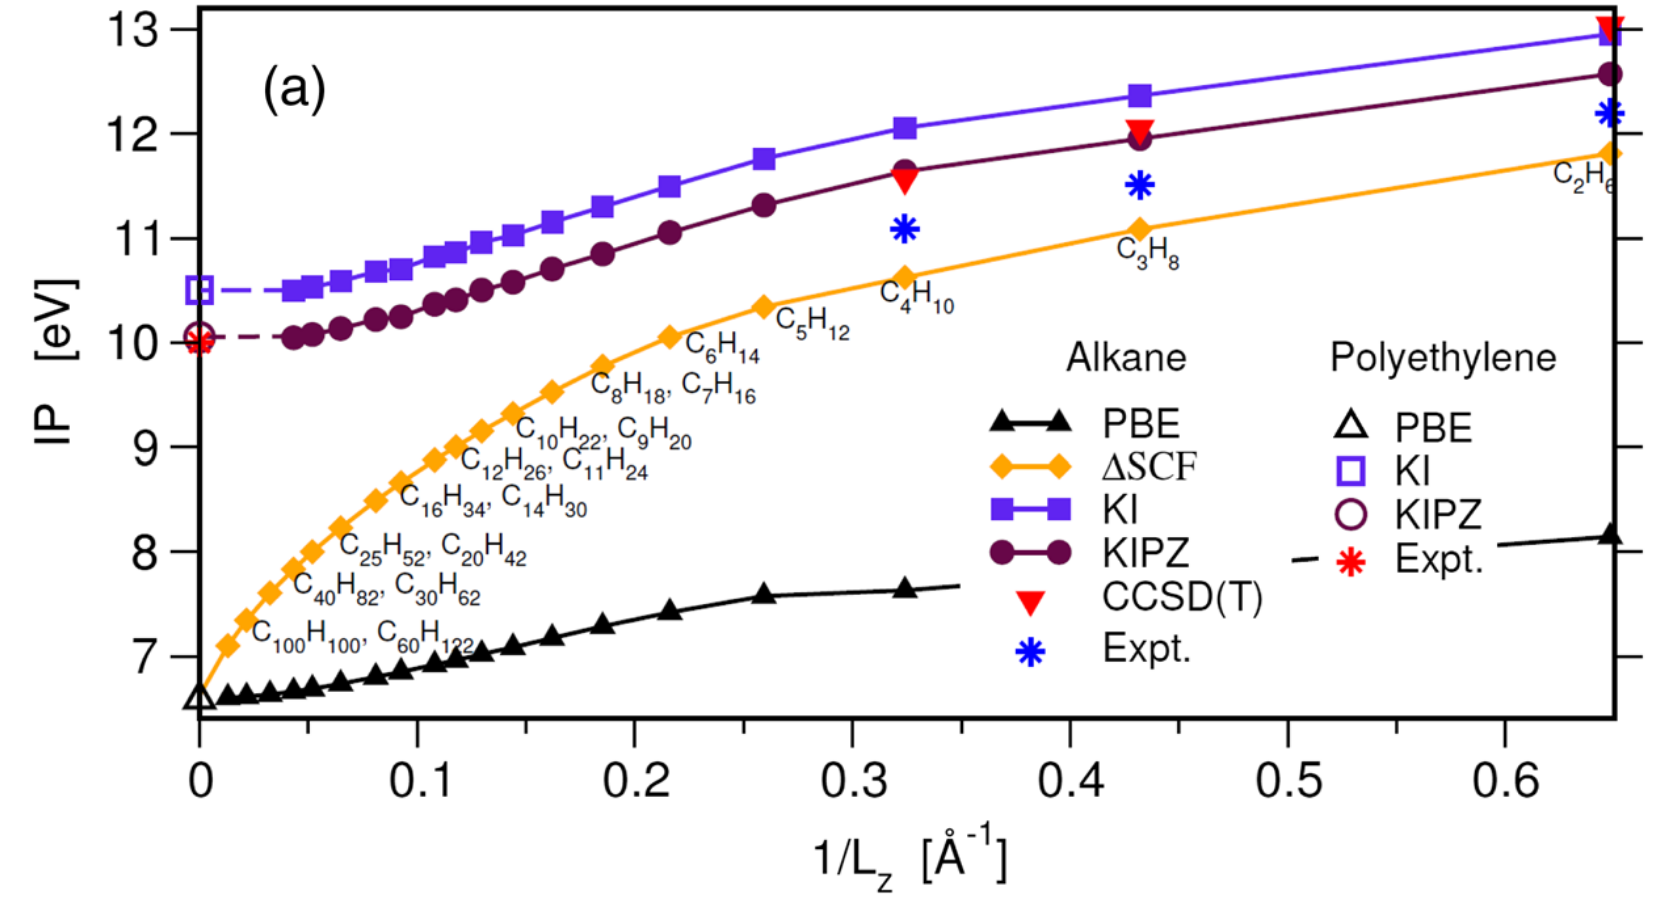
\includegraphics[width=0.6\textwidth]{figures/nguyen_bulk_limit.png}
   \end{center}
   \blfootcite{Nguyen2018}

   \vspace{-2ex}

   \begin{overlayarea}{\textwidth}{0.25\textheight}
      \only<2-3>{
         In the bulk limit for one cell $\Delta E = E(N-\delta N) - E(N)$
      }%

      \only<3>{
         Across all the cells $
            \Delta E = \frac{1}{\delta N}\left(E(N-\delta N) - E(N)\right) = -\frac{dE}{dN} = -\varepsilon_\mathsf{HO}$
      }%
      \only<4->{
         \begin{equation*}
            \lim_{n_i(r) \rightarrow 0}
            v^\mathsf{KI}_{{i}}/\alpha_i =
            \lim_{n_i(r) \rightarrow 0}
            - E_{\mathsf{H}}\left[{n_{i}}\right]
            + E_{\mathsf{xc}}\left[\rho\right]
            - E_{\mathsf{xc}}\left[\rho-{n_{i}}\right]
            - \int d\mathbf{r'}
            v_\mathsf{xc}(\mathbf{r}', [\rho])
            {n_{i}}(\mathbf{r}')
            = 0
         \end{equation*}
      }%
   \end{overlayarea}
\end{frame}

\begin{frame}{Orbital-density-dependence}
   Other features of orbital-density-dependence
   \begin{itemize}[<+(1)->]
      \item ODD functional means that we know $\hat H \ket{\varphi_i}$ for variational orbitals $\{\ket{\varphi_i}\}$ but we don't know $\hat H$ in general
      \item Practically we can often use MLWFs
      \item a natural generalisation in the direction of spectral functional theory (as discussed already by Andrea)\footcite{Ferretti2014}
   \end{itemize}

\end{frame}

\begin{frame}{Screening}
   \small
   \begin{itemize}[<+->]
      \item In Hartree-Fock (the original ``Koopmans' theorem''):
            \begin{equation*}
               E^{HF}_{ee} = \frac{1}{2}\sum_{ij} f_i f_j \int d\mathbf{r} d\mathbf{r}' \frac{|\psi_i(\mathbf{r})|^2|\psi_j(\mathbf{r'})|^2}{\mathbf{r} - \mathbf{r}'} - \frac{\psi_i^*(\mathbf{r})\psi_j^*(\mathbf{r'})\psi_i(\mathbf{r'})\psi_j(\mathbf{r})}{\mathbf{r} - \mathbf{r}'}
            \end{equation*}
            \blfootcite{Li2017}
      \item Account for screening post-hoc:
            \begin{equation*}
               \frac{d E}{d f_i}
               \approx
               \alpha_i
               \frac{\partial E}{\partial f_i}
            \end{equation*}
      \item How to choose an appropriate value for $\alpha_i$? Return to the original idea of Koopmans functionals:
            \begin{equation*}
               \varepsilon_i^\mathsf{Koopmans} = E_i(N-1) - E(N)
            \end{equation*}
   \end{itemize}

\end{frame}

\begin{frame}{Screening}

   \begin{overlayarea}{\textwidth}{0.65\textheight}
      \begin{center}
         \only<1>{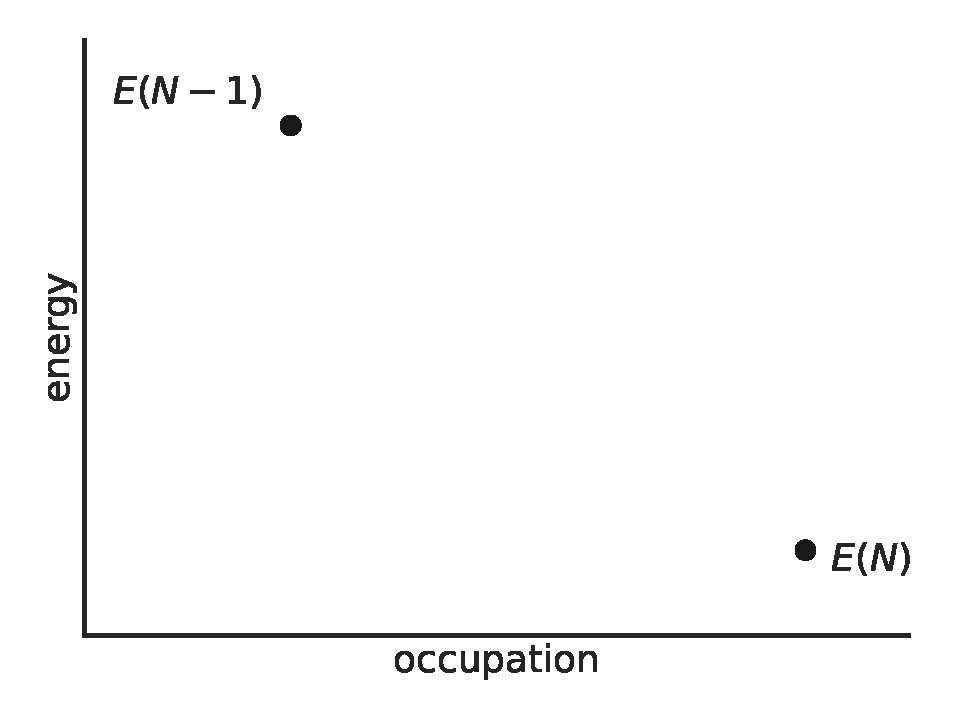
\includegraphics[width=0.5\textwidth]{figures/alpha_calc/fig_alpha_calc_step_0.pdf}}%
         \only<2>{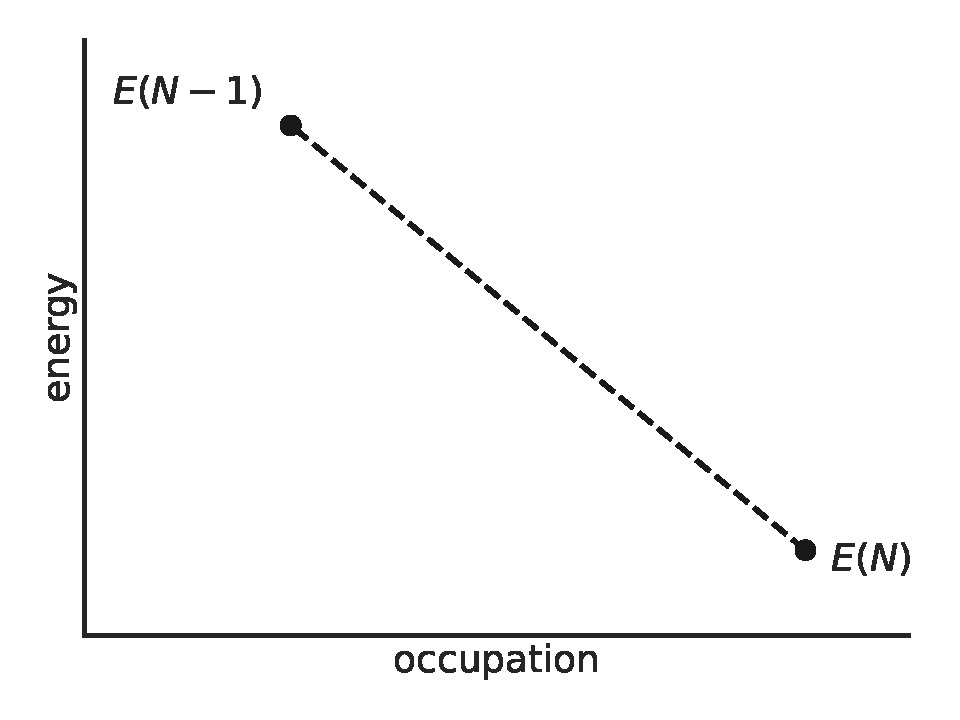
\includegraphics[width=0.5\textwidth]{figures/alpha_calc/fig_alpha_calc_step_1.pdf}}%
         \only<3-4>{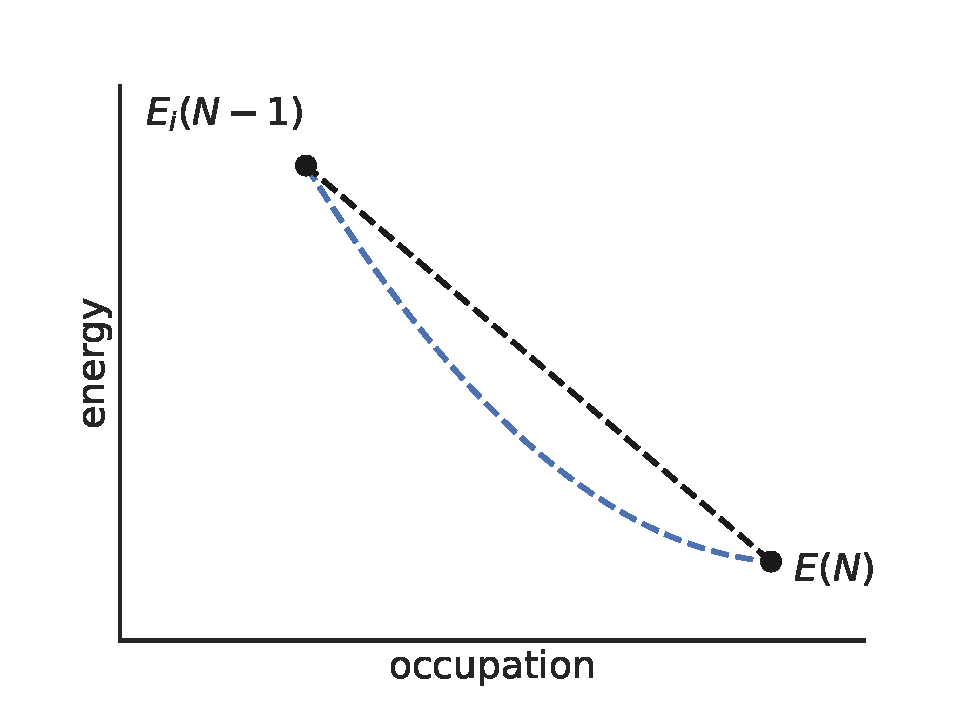
\includegraphics[width=0.5\textwidth]{figures/alpha_calc/fig_alpha_calc_step_2.pdf}}%
         \only<5>{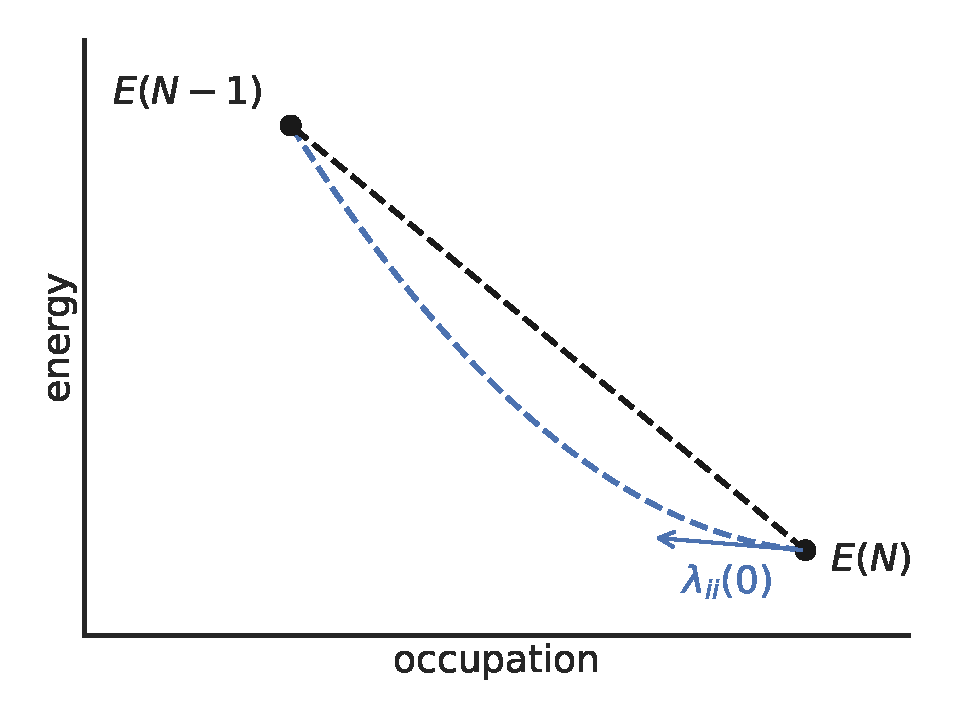
\includegraphics[width=0.5\textwidth]{figures/alpha_calc/fig_alpha_calc_step_3.pdf}}%
         \only<6->{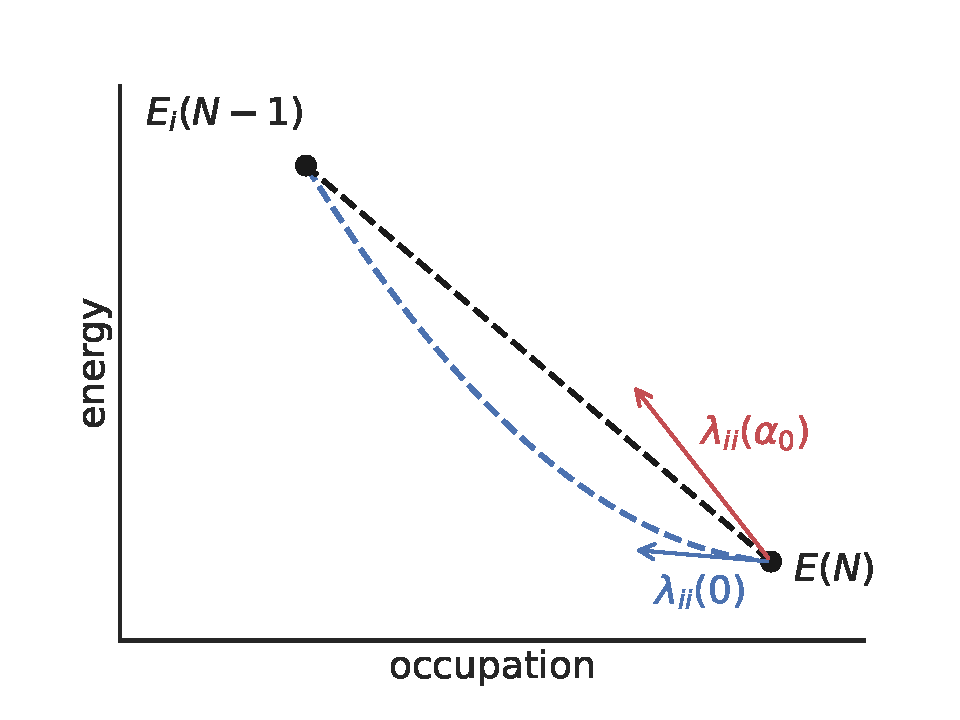
\includegraphics[width=0.5\textwidth]{figures/alpha_calc/fig_alpha_calc_step_4.pdf}}%
      \end{center}

   \end{overlayarea}

   \begin{overlayarea}{\textwidth}{0.3\textheight}
      \only<4-6>{
         \begin{equation*}
            \lambda_{ii}(\alpha) \equiv
            \braopket{\varphi_i}{\hat h^\mathsf{DFT} + \alpha \hat v^\mathsf{Koopmans}}{\varphi_i}
            =
            \left.\frac{dE^\mathsf{Koopmans}}{df_i}\right|_{f_i = s}
         \end{equation*}
      }
      \only<7->{Given this, how to work out the ideal $\alpha$?}
      \only<8->{
         \begin{equation*}
            \alpha_{n+1} = \alpha_{n} \frac{E_i(N-1) - E(N) - \lambda_{ii}(0)}{\lambda_{ii}(\alpha_{n}) - \lambda_{ii}(0)}
         \end{equation*}
      }
   \end{overlayarea}
\end{frame}

\begin{frame}{Screening}
   \begin{equation*}
      \alpha^{n+1} = \tikzmarknode{alpha}{\alpha^{n}} \frac{\tikzmarknode{enm1}{E_i(N-1)} - \tikzmarknode{en}{E(N)} - \lambda_{ii}(0)}{\tikzmarknode{lambdaa}{\lambda_{ii}(\alpha^{n})} - \tikzmarknode{lambda0}{\lambda_{ii}(0)}}
   \end{equation*}
   \begin{tikzpicture}[overlay,remember picture,seaborn_red,>=stealth,shorten
         <=0.2ex,nodes={font=\footnotesize,align=left,inner ysep=1pt},<-]
      \onslide<2->{
         \draw (lambdaa.south) -- ++ (0,-4em) node[anchor=north,align=center]
         (lambdaatext) {expectation value \\ of $\hat{H}^\mathsf{Koopmans}$};
      }
      \onslide<3->{
         \draw (lambda0.south) -- ++ (0,-1.5em) node[anchor=north,align=center]
         (lambda0text) {expectation value \\ of $\hat{H}^\mathsf{DFT}$};
      }
      \onslide<4->{
         \draw (en.north) -- ++ (0,1.5em) node[anchor=south,align=center]
         (entext) {total energy \\ of neutral system};
      }
      \onslide<5->{
         \draw (enm1.north) -- ++ (0,4em) node[anchor=south,align=center]
         (enm1text) {total energy with electron \\ removed from orbital $i$};
      }
   \end{tikzpicture}
\end{frame}

\begin{frame}{Screening via DFPT}
   How can we avoid explicit charged defect calculations in a supercell?

   \onslide<2->{
   Reformulate in terms of DFPT\footcite{Colonna2019}...

   \begin{equation*}
   \alpha_{i} = 1 + \frac{\langle v^{i}_{\rm pert} \vert \Delta^{i} n \rangle}{\langle n_{i} \vert v^{i}_{\rm pert} \rangle}.
   \end{equation*}
   }
   
   \onslide<3->{
   ... in reciprocal space\footcite{Colonna2022}
   \begin{equation*}
      \alpha_{\mathbf{0}i} =  1 + \frac{\sum_{\mathbf{q}} \langle v^{\mathbf{0}i}_{\rm pert,\mathbf{q}} \vert \Delta^{\mathbf{0}i}_{\mathbf{q}}n \rangle} {\sum_{\mathbf{q}} \langle n^{\mathbf{0}i}_{\mathbf{q}} \vert v^{\mathbf{0}i}_{\rm pert,\mathbf{q}} \rangle}.
   \end{equation*}

   (See Nicola Colonna's talk)
   }

   \vspace{1ex}
   \onslide<4->{N.B. even for the supercell, we can still reconstruct a band structure\footcite{DeGennaro2022}}

\end{frame}

\begin{frame}{To summarise...}

   When performing a Koopmans calculation, you must decide...
   \begin{itemize}[<+(1)->]
      \item which flavour (KI, KIPZ)?
      \item how are we treating the orbital-density-dependence?
      \begin{itemize}
         \item how are we initialising our variational orbitals? (N.B. depends on the flavour!)
         \item are we going to explicitly minimise the ODD?
      \end{itemize}
      \item how are we calculating the screening parameters? (finite differences, DFPT, ML...)
   \end{itemize}
   
\end{frame}


\begin{frame}{Koopmans functionals: results for molecules}
   \small
   Ionisation potentials of 100 molecules cf. CCSD(T)
   \begin{center}
      \includegraphics[height=0.2\textwidth]{figures/colonna_2019_gw100_ip}
      % \onslide<2->{\includegraphics[height=0.23\textwidth]{figures/colonna_2019_gw100_deeper}}
   \end{center}

   \vspace{-3ex}
   Ultraviolet photoemission spectra
   \begin{center}
      \begin{tikzpicture}
         \node [inner sep=0pt](fig) at (0,0) {\includegraphics[height=0.35\textheight]{figures/fig_nguyen_prl_spectra.png}};
         \draw [very thick, color=seaborn_red] (-5.35,-0.07) rectangle (5.4,1.6);
      \end{tikzpicture}
   \end{center}
   \vspace{-2ex}

   \blfootcite{Colonna2018,Nguyen2015}
\end{frame}

\begin{frame}{Koopmans functionals: results for solids}
   \begin{minipage}[c]{0.35\textwidth}
      \includegraphics[width=\textwidth]{figures/fig_nguyen_prx_bandgaps.png}
   \end{minipage}
   \hspace{1em}
   \begin{minipage}[c]{0.6\textwidth}

      \footnotesize
      Mean absolute error (eV) across prototypical semiconductors and insulators

      \vspace{1ex}
      \begin{tabular}{c S[table-format = 2.2] S[table-format = 2.2] >{\color{seaborn_red}\bfseries}S[table-format = 2.2] >{\color{seaborn_red}\bfseries}S[table-format = 2.2] S[table-format = 2.2]}
                          & {PBE} & {G\textsubscript{0}W\textsubscript{0}} & {KI} & {KIPZ} & {QSG$\tilde{\mathrm{W}}$} \\
         \midrule
         \midrule
         $E_\mathrm{gap}$ & 2.54  & 0.56                                   & 0.27 & 0.22   & 0.18                      \\
         %                                  & {MAPE (\%)} & 48.28 & 12.10      & 7.0           \\
         \midrule
         IP               & 1.09  & 0.39                                   & 0.19 & 0.21   & 0.49                      \\
         %                                  & {MAPE (\%)} & 15.58 & 5.71                                   & 2.99 & 3.14   & 7.41
      \end{tabular}
   \end{minipage}

   \blfootcite{Nguyen2018}
\end{frame}

\begin{frame}{Koopmans functionals: results for solids}
   
\begin{table}[t]
   \centering
   \footnotesize
   \begin{tabular}{r@{ $\rightarrow$ } l *{3}{d{2.2}} >{\color{seaborn_red}}S[table-format = 2.2] >{\color{seaborn_red}}S[table-format = 2.2] d{2.2} @{$\pm$} d{1.2}}
      \hline
      \hline
      \multicolumn{2}{c}{ }
                                & \multicolumn{1}{c}{PBE}
                                & \multicolumn{1}{c}{G\textsubscript{0}W\textsubscript{0}\footnote{\cite{Shishkin2007} for $E_g$ and \cite{Hybertsen1986} for the transitions;}}
                                & \multicolumn{1}{c}{scG$\tilde{\mathrm{W}}$\footcite{Shishkin2007a}}
                                & \multicolumn{1}{c}{
                                 \textcolor{seaborn_red}{\bfseries KI@[PBE,MLWFs]}}
                                & \multicolumn{1}{c}{
                                 \textcolor{seaborn_red}{\bfseries KIPZ@PBE}}
                                & \multicolumn{2}{c}{exp\footcite{Madelung2004}}                                                                                                                                                                   \\
      \hline
      \multicolumn{2}{c}{$E_g$} &
      0.49 &  1.06 & 1.14 &  1.16 &   1.15 & \multicolumn{2}{c}{1.17}\\
      $\Gamma_{1v}$ & $\Gamma_{25'v}$ & 11.97 & 12.04 &      & 11.97 & 12.09 & 12.5 &  0.6\\
      $X_{1v}$ & $\Gamma_{25'v}$ &  7.82 &       &      &  7.82       &       & \multicolumn{2}{c}{7.75}\\
      $X_{4v}$ & $\Gamma_{25'v}$ &  2.85 &  2.99 &      &  2.85 & 2.86 & \multicolumn{2}{c}{2.90}\\
      $L_{2'v}$ & $\Gamma_{25'v}$ &  9.63 &  9.79 &      &  9.63 &  9.74 &  9.3 &  0.4\\
      $L_{1v}$ & $\Gamma_{25'v}$ &  6.98 &  7.18 &      &  6.98 &   7.04 &  6.8 &  0.2\\
      $L_{3'v}$ & $\Gamma_{25'v}$ &  1.19 &  1.27 &      &  1.19 &       &  1.2 &  0.2\\
      $\Gamma_{25'v}$ &  $\Gamma_{15c}$ &  2.48 &  3.29 &      &  3.17  &  3.20 & 3.35 & 0.01\\
      $\Gamma_{25'v}$ &  $\Gamma_{2'c}$ &  3.28 &  4.02 &      &  3.95  &  3.95 & 4.15 & 0.05\\
      $\Gamma_{25'v}$ &        $X_{1c}$ &  0.62 &  1.38 &      &  1.28  &  1.31 & \multicolumn{2}{c}{1.13} \\
      $\Gamma_{25'v}$ &        $L_{1c}$ &  1.45 &  2.21 &      &  2.12  &  2.13 & 2.04 & 0.06\\
      $\Gamma_{25'v}$ &        $L_{3c}$ &  3.24 &  4.18 &      &  3.91  &  3.94 &  3.9 &  0.1\\
      \hline
      \multicolumn{2}{c}{MSE} & 0.35 &  0.02 &      &  0.01 &   0.03\\
      \multicolumn{2}{c}{MAE} & 0.44 &  0.21 &      &  0.14 &   0.17\\
      \hline
      \hline
   \end{tabular}

   % \textsuperscript{\emph{a}} this work;
   % \textsuperscript{\emph{b}} Ref.~\citenum{Shishkin2007} for $E_g$ and Ref.~\citenum{Hybertsen1986} for the transitions;
   % \textsuperscript{\emph{c}} Ref.~\citenum{Shishkin2007a};
   % \textsuperscript{\emph{d}} Ref.~\citenum{DeGennaro2022};
   % \textsuperscript{\emph{e}} Ref.~\citenum{Madelung2004}
\end{table}
\end{frame}
\begin{frame}{Koopmans functionals: results for toy systems}
   For Hooke's atom (two electrons in a harmonic confining potential with Coulombic repulsion)

   \begin{figure}[t]
      \begin{subfigure}{0.4\textwidth}
         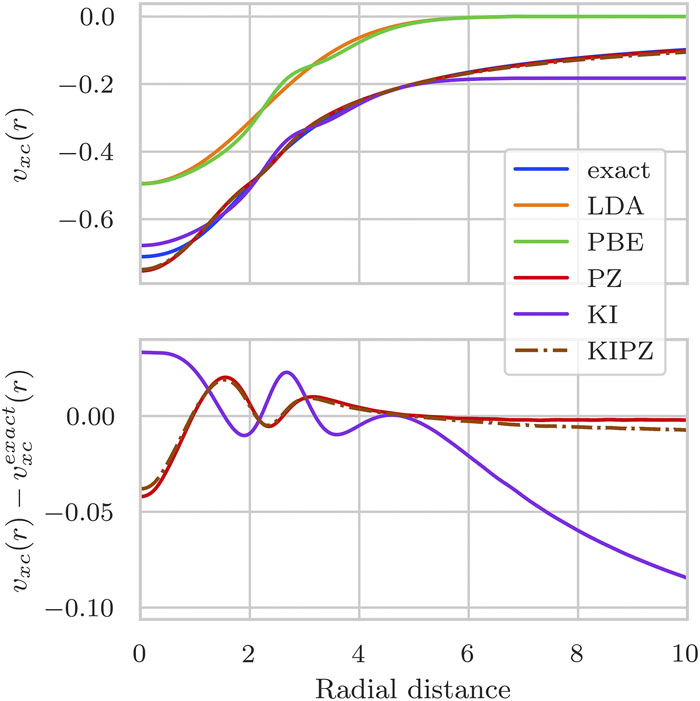
\includegraphics[width=\columnwidth]{figures/schubert_vxc.jpeg}
      \end{subfigure}
      \begin{subfigure}{0.4\textwidth}
         \onslide<2->{
         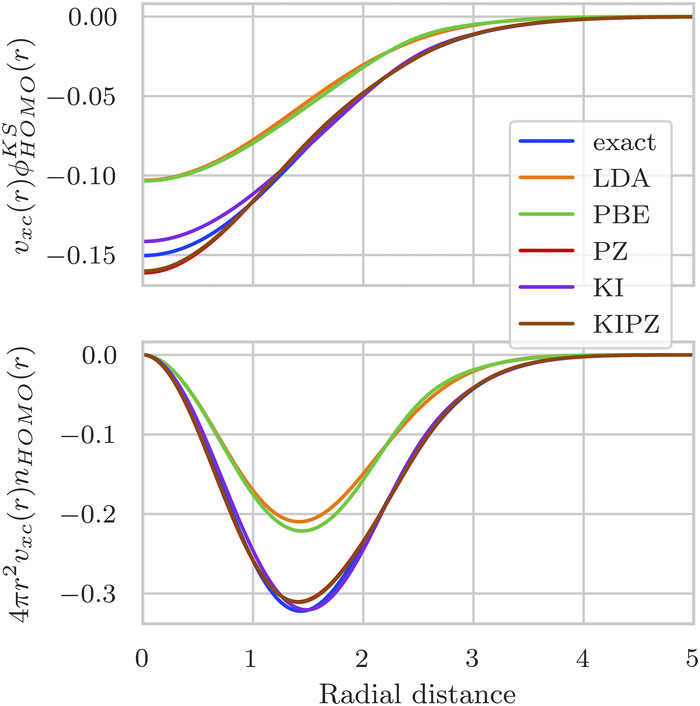
\includegraphics[width=\columnwidth]{figures/schubert_vxc_integrated.jpeg}
         }
      \end{subfigure}
   \end{figure}

   \blfootcite{Schubert2023}
\end{frame}

\begin{frame}{Koopmans functionals: caveats}

   \begin{itemize}[<+(1)->]
      \item restricted to systems with a non-zero band gap
      \item empty state localization in the bulk limit
      \item can potentially break the crystal point group symmetry\blfootcite{Su2020}
   \end{itemize}
\end{frame}

\begin{frame}{The workflows}
   The general workflow:
   \begin{itemize}
      \item define/initialize a set of variational orbitals
      \item calculate the screening parameters $\{\alpha_i\}$
      \item construct and diagonalize the Hamiltonian
   \end{itemize}
\end{frame}

\begin{frame}{The workflows}

   \vspace{1ex}

   \onslide<1->{
      (a) finite difference calculations using a supercell

      \vspace{-2ex}
      \adjustbox{width=\textwidth}{\begin{tikzpicture}[font=\tiny, x=3.5cm, y=1cm]
\begin{pgfonlayer}{background}
   % \node[fit= (KC init) (empty label) (filled label) (sc loop 1) (converged label), fill=seaborn_bg_grey, inner sep=0.5cm] (calculating screening) {};
   % \node [dummy, above=0cm of calculating screening, font=\sffamily]{Calculating screening parameters};
   \fill [seaborn_bg_grey_dark] (-2.1,-0.8) rectangle (1.3,4.6);
   \node at (-2.1, 4.6) [default_text] {\large Initialisation (molecules)};
   \fill [seaborn_bg_grey_dark] (-2.1,-4.6) rectangle (1.3,-1.2);
   \node at (-2.1, -1.2) [default_text] {\large Initialisation (solids)};
   \fill [seaborn_bg_grey_dark] (1.4,-4.6) rectangle (6.9,4.6);
   \node at (1.4, 4.6) [default_text] {\large Calculating screening parameters};
   \fill [seaborn_bg_grey_dark] (7,-4.6) rectangle (8,4.6);
   \node at (7, 4.6) [default_text, text width=3.5cm] {\large Final calculation};
   \fill [seaborn_bg_grey_dark] (8.1,-4.6) rectangle (9.1,4.6);
   \node at (8.1, 4.6) [default_text, text width=3.5cm] {\large Postprocessing (solids)};
\end{pgfonlayer}

    % Key
    \node at (6.85, 5.25) [cp, text width=1.4cm, minimum height=0.7cm] {\texttt{cp}};
    \node at (7.35, 5.25) [pw, text width=1.4cm, minimum height=0.7cm] {\texttt{pw}};
    \node at (7.85, 5.25) [wannier90, text width=1.4cm, minimum height=0.7cm] {\texttt{wannier90}};
    \node at (8.35, 5.25) [bespoke, text width=1.4cm, minimum height=0.7cm, font=\tiny] {bespoke code};
    \node at (8.85, 5.25) [observable, text width=1.4cm, minimum height=0.7cm, font=\tiny] {quantity of interest};
    
    % Initialisation
    % Option 1
    \node at (-1, 2.9) [cp] (PBE init) {PBE};
    \node at (0, 2.9) [cp] (PZ innerloop) {PZ unitary rotation};
    \path [line] (PBE init) -- (PZ innerloop);
    
    % OR
    \node at (-0.5, 1.9) [default] (or) {or};
    
    % Option 2
    \node at (-0.5, 0.9) [cp] (PZ init) {PZ};
    
    % Solids
    \node at (-1.5, -2.9) [pw] (pw PBE init) {PBE (primitive cell)};
    \node at (-0.5, -2.9) [wannier90] (wannierize) {wannierize};
    \node at (0.5, -2.9) [bespoke] (unfold) {fold to supercell};
    \path [line] (pw PBE init) -- (wannierize);
    \path [line] (wannierize) -- (unfold);
    
    % Calculating screening parameters
    \node at (2, 0) [cp] (KC init) {$\alpha_0$KI/$\alpha_0$KIPZ};
    
    \path let
    \p1 = (PZ innerloop),
    \p2 = (unfold.east)
    in
    coordinate (dummy) at (\x2, \y1);
    \path let
    \p1 = (PZ init),
    \p2 = (unfold.east)
    in
    coordinate (dummy2) at (\x2, \y1);
    \path [line] (PZ innerloop) -- (dummy) to[-|-=0.3] ([yshift=2\myyshift]KC init.west);
    \path [line] (PZ init.east) -- ([xshift=-3.5\myyshift]dummy2) to[-|-=0.3] (KC init.west);
   \path [line] (unfold.east) to[-|-=0.3] ([yshift=-2\myyshift]KC init.west);
    
    % KI filled %%%%%%%%%%%%%%%%%%%%%%%%%%%%%%%%%%%%%%%%%%%%%%%%%%
    
    % calculations
    \node at (3, 3) [cp] (N-1_filled) {PBE/$\alpha_0$KIPZ ($N-1$)};
   % \node at (3, 2) [cp] (PBE_filled) {PBE};
   % \node at (3, -2) [cp] (PBE_empty) {PBE};
    \node at (3, -3) [cp] (N+1_empty) {PBE/$\alpha_0$KIPZ ($N+1$)};
    
   % \path [line] (KC init) to[-|-] (PBE_filled);
    \path [line] (KC init) to[-|-] (N-1_filled);
   % \path [line] (KC init) to[-|-] (PBE_empty);
    \path [line] (KC init) to[-|-] (N+1_empty);
    
    % results
    \node at (4, 3) [observable] (EN-1_filled) {$E_i(N-1)$};
    \node at (4, 2) [observable] (lambda0_filled) {$\lambda^{0}_{ii}(1)$};
    \node at (4, 1) [observable] (lambda_filled) {$\lambda^{\alpha_0}_{ii}(1)$};
    \node at (4, 0) [observable] (EN) {$E(N)$};
    \node at (4, -1) [observable] (lambda_empty) {$\lambda^{\alpha_0}_{ii}(0)$};
    \node at (4, -2) [observable] (lambda0_empty) {$\lambda^{0}_{ii}(0)$};
    \node at (4, -3) [observable] (EN+1_empty) {$E_i(N+1)$};
    
    \path [line] (KC init) -- (EN);
    \path [line] (KC init.east) to[-|-] (lambda_filled.west);
    \path [line] (KC init.east) to[-|-] (lambda_empty.west);
   \path [line] (KC init.east) to[-|-] (lambda0_filled.west);
   \path [line] (KC init.east) to[-|-] (lambda0_empty.west);
    
   % \path [line] (PBE_filled) -- (lambda0_filled);
    \path [line] (N-1_filled) -- (EN-1_filled);
    
   % \path [line] (PBE_empty) -- (lambda0_empty);
    \path [line] (N+1_empty) -- (EN+1_empty);
    
    % alpha parameters
    \node at (5, 1.5) [observable] (alpha filled) {$\alpha_{i \in \text{filled}}$};
    \node at (5, -1.5) [observable] (alpha empty) {$\alpha_{i \in \text{empty}}$};
    
    \path [line] (lambda_filled) to[-|-] (alpha filled);
    \path [line] ([yshift=\myyshift]EN.east) to[-|-] (alpha filled.west);
    \path [line] (lambda0_filled) to[-|-] (alpha filled);
    \path [line] (EN-1_filled) to[-|-] (alpha filled);
    
    \path [line] (lambda_empty) to[-|-] (alpha empty);
    \path [line] ([yshift=-\myyshift]EN.east) to[-|-] (alpha empty.west);
    \path [line] (lambda0_empty) to[-|-] (alpha empty);
    \path [line] (EN+1_empty) to[-|-] (alpha empty);
    
    % SC check
    \coordinate (sc check) at (6, 0);
    \path [headless_line] (alpha empty) to[-|-] (sc check);
    \path [headless_line] (alpha filled) to[-|-] (sc check);
    
    % SC loop
    \node [below= of EN+1_empty] (sc loop y) {};
    \path let
    \p1 = (sc check),
    \p2 = (sc loop y)
    in
    coordinate (sc loop 1) at (\x1, \y2);
    \path [line] (sc check) -- node [midway, right, font=\sffamily] (not converged label) {\footnotesize $\{\alpha_i\}$ not converged} (sc loop 1) -| (KC init.south);
    
    % Final calc
    \node at (7.5, 0) [cp] (final KI) {$\alpha$KI/$\alpha$KIPZ};
    \path [line] (sc check) -- node [midway, above, font=\sffamily] (converged label) {\footnotesize $\{\alpha_i\}$ converged} (final KI);
    
    % Postproc
    \node at (8.6, 0) [bespoke] (upfold) {unfold to primitive cell};
    \path [line] (final KI) -- (upfold);
    
    % Boxes
    % Screening parametere
   \node [boxwhite, fit= (N-1_filled) (EN-1_filled),
       draw, dashed, fill opacity=0, inner sep=0.35cm](filled box){};
   \node [dummy, above=0cm of filled box, font=\sffamily](filled label){\footnotesize one per filled orbital (index $i$)};
   \node [boxwhite, fit= (N+1_empty) (EN+1_empty),
       draw, dashed, fill opacity=0, inner sep=0.35cm](empty box){};
   \node [dummy, below=0cm of empty box, font=\sffamily](empty label){\footnotesize one per empty orbital (index $i$)};
    
    % \onslide<2->{
    %    \node at (3.5, 0) [default_text, fill=white, opacity=0.9, text opacity=1, anchor=center, minimum height=5cm, text width=7.5cm, execute at begin node=\setlength{\baselineskip}{30pt}] (nc text) {
    %       \huge Riccardo De Gennaro
    %       \textbf{M22.00004} / paper in preparation
    %    };
    %    \node[right = -0.2cm of nc text, anchor=west]{\includegraphics[height=5cm]{figures/riccardo_degennaro.jpg}};
    % }
    
    
    % ML
\end{tikzpicture}}
   }

   \vspace{-1.5ex}
   \onslide<2->{
      (b) DFPT in a primitive cell

      \vspace{-2ex}
      \adjustbox{width=0.655\textwidth}{\begin{tikzpicture}[font=\tiny, x=3.5cm, y=1cm]
   \begin{pgfonlayer}{background}
      \fill [seaborn_bg_grey_dark] (-2.2,-1) rectangle (1.2,1.5);
      \node at (-2.2, 1.5) [default_text] {\large Initialisation};
      \fill [seaborn_bg_grey_dark] (1.3,-1) rectangle (3.7,1.5);
      \node at (1.3, 1.5) [default_text] {\large Calculating screening parameters};
      \fill [seaborn_bg_grey_dark] (3.8,-1) rectangle (5.2,1.5);
      \node at (3.8, 1.5) [default_text, text width=3.5cm] {\large Final calculation};
      % \fill [seaborn_bg_grey_dark] (8.1,-1) rectangle (9.1,1.5);
      % \node at (8.1, 1.5) [default_text, text width=3.5cm] {\large Postprocessing};
   \end{pgfonlayer}

   % Key
   \node at (3.45, 2.15) [pw, text width=1.4cm, minimum height=0.7cm] {\texttt{pw\vphantom{0}}};
   \node at (3.95, 2.15) [wannier90, text width=1.4cm, minimum height=0.7cm] {\texttt{w90}};
   \node at (4.45, 2.15) [kcw, text width=1.4cm, minimum height=0.7cm] {\texttt{kcw}};
   \node at (4.95, 2.15) [observable, text width=1.4cm, minimum height=0.7cm, font=\tiny\sffamily] {quantity of interest};

   % Initialisation
   % Solids
   \node at (-1.5, 0) [pw] (pw DFT init) {DFT};
   \node at (-0.5, 0) [wannier90] (wannierize) {wannierize};
   \node at (0.5, 0) [kcw] (w2k) {Wannier function conversion};
   \path [line] (pw DFT init) -- (wannierize);
   \path [line] (wannierize) -- (w2k);

   % Calculating screening parameters
   \node at (2, 0) [kcw] (KC screen) {DFPT calculation};
   \node at (3, 0) [observable] (alphas) {$\{\alpha_i\}$};
   \path [line] (w2k) -- (KC screen);
   \path [line] (KC screen) -- (alphas);

   % Final calc
   \node at (4.5, 0) [kcw] (KC ham) {$\alpha_0$KI/$\alpha_0$KIPZ};
   \path [line] (alphas) -- (KC ham);

\end{tikzpicture}
}
   }
   % \onslide<6>{
   %    \vspace{-0.375\paperheight}
   %    \begin{flushright}
   %       \begin{tcolorbox}[enhanced jigsaw, width=4cm, opacityback=0, colframe=seaborn_red, coltext=seaborn_red, left=3pt, bottom=3pt, top=3pt, right=3pt, tikz={rotate=30,transform shape}, boxrule=1.5mm]
   %          \begin{center}
   %             \includegraphics[height=1cm]{./figures/qe_logo_high_res_cropped.jpg}
   %             \bf \huge\ \raisebox{0.3cm}{+}\,
   %             \includegraphics[height=1cm]{./figures/python_logo.png}

   %             \bf \large OUT NOW!
   %          \end{center}
   %       \end{tcolorbox}
   %    \end{flushright}
   % }

\end{frame}

% \begin{frame}{Koopmans compared to DFT+\emph{U}}
%    \small
%    \renewcommand{\arraystretch}{1.5}
%    \rowcolors{1}{seaborn_bg_grey}{seaborn_bg_grey_half}
%    \begin{tabularx}{\columnwidth}{L L L}
%                                    & \textbf{DFT+\emph{U}}                                                       & \textbf{Koopmans}                                                                                                           \\
%       \hline
%       % designed to correct SIE, as defined by... & erroneous global curvature in total energies                                & dependence of $\varepsilon_i$ on $f_i \ \forall i$ \leavevmode\onslide<4->{\textcolor{red}{(canonical orbitals)}}                                                   \\
%       the functional...            & corrects local curvature in total energies                                  & \leavevmode\onslide<2->{removes dependence of $\varepsilon_i$ on $f_i$ and guarantees $\varepsilon_i = E_i(N\pm 1) - E(N)$} \\
%       correction applied to...     & selected subspaces only (e.g. \emph{3d} orbitals)                           & \leavevmode\onslide<3->{every variational orbital in the entire system}                                                     \\
%       orbitals defined by...       & Hubbard projectors (atom-centred, frozen, incomplete)                       & \leavevmode\onslide<4->{variational (minimising) orbitals}                                                                  \\
%       corrective parameters are... & $\{U^I\}$, defined with respect to charge-neutral excitations (if using LR) & \leavevmode\onslide<5->{$\{\alpha_i\}$, defined with respect to charged excitations}                                        \\
%    \end{tabularx}
% \end{frame}

% \begin{frame}{Implementations of Koopmans functionals}
% 
%    \texttt{kcw.x} (DFPT implementation) is distributed in Quantum ESPRESSO v7.1 onwards
% 
%    \vspace{2ex}
% 
%    \texttt{kcp.x} (supercell implementation) is available publically
% 
%    \vspace{2ex}
%    \small
%    \renewcommand{\arraystretch}{1.5}
%    \rowcolors{1}{seaborn_bg_grey}{seaborn_bg_grey_half}
%    \begin{tabularx}{\columnwidth}{L L L}
%                                    & \textbf{\texttt{kcw.x}}                                                       & \textbf{\texttt{kcp.x}}                                                                                                          
%       \onslide<2->{\\ \hline available flavours            & KI only & KI, KIPZ, pKIPZ, PZ}
%       \onslide<3->{\\ screening parameters...     & DFPT & finite differences}
%       \onslide<4->{\\ $k$-point sampling         & explicit & implicit (via supercell)}
%       \onslide<5->{\\ orbital minimization & uses MLWFs as a proxy (approximate) & explicit}
%       \onslide<6->{\\ scaling & $\mathcal{O}(N_\mathbf{q}N_\mathbf{k}N_\mathsf{orb}^3)$ & $\mathcal{O}(N_\mathbf{k}^3 N_\mathsf{orb}^3) = \mathcal{O}(N_k) \times $ primitive cell approach}
%    \end{tabularx}
%    
% \end{frame}

\begin{frame}{How do I run these calculations?}
   Complicated workflows mean that...
   \begin{itemize}[<+(1)->]
      \item lots of different codes that need to handshake
      \item lots of scope for human error
      \item reproducibility becomes difficult
      \item expert knowledge required
   \end{itemize}

   \onslide<6>{Our solution...}

\end{frame}

\begin{frame}{}
   \begin{center}
      \includegraphics[width=0.6\textwidth]{figures/koopmans_grey_on_transparent.png}
   \end{center}

   \vspace{-2ex}

   \begin{columns}
      \begin{column}{0.55\textwidth}
         \begin{itemize}
            \item v1.0 released earlier this year\footnotemark[1]
            \item implementations of Koopmans functionals
            \item automated workflows
                  \begin{itemize}
                     \item start-to-finish Koopmans calculations
                     \item Wannierisation
                     \item dielectric tensor
                     \item ...
                  \end{itemize}
            \item built on top of ASE\footnotemark[2]
            \item under the hood, calls \texttt{Quantum ESPRESSO}
            \item does not require expert knowledge
         \end{itemize}
      \end{column}

      \begin{column}{0.4\textwidth}
         \centering
         \url{koopmans-functionals.org}
         \includegraphics[width=\columnwidth]{figures/website_cropped.png}
      \end{column}
   \end{columns}
   \footnotetext[1]{\cite{Linscott2023}}
   \footnotetext[2]{\cite{Larsen2017}}
\end{frame}

\begin{frame}{koopmans: the input file}
   \begin{minipage}[t]{0.475\columnwidth}
      \inputminted[fontsize=\tiny,breaklines,lastline=20]{json}{scripts/si.json}
   \end{minipage}
   \hspace{0.025\textwidth}
   \begin{minipage}[t]{0.475\columnwidth}
      \inputminted[fontsize=\tiny,breaklines,firstline=21]{json}{scripts/si.json}
   \end{minipage}
\end{frame}

% \begin{frame}{koopmans: the output file}
%    \vspace{-2ex}
%    \only<1>{
%       \inputminted[fontsize=\scriptsize,breaklines]{text}{scripts/si_ki_full.out}
%    }
%    \only<2>{
%       \inputminted[fontsize=\scriptsize,breaklines,firstline=25]{text}{scripts/si_ki_full.out}
%    }
%    \only<3>{
%       \inputminted[fontsize=\scriptsize,breaklines,firstline=50]{text}{scripts/si_ki_full.out}
%    }
%    \only<4>{
%       \inputminted[fontsize=\scriptsize,breaklines,firstline=75]{text}{scripts/si_ki_full.out}
%    }
% \end{frame}

\begin{frame}{koopmans is scriptable}
   \vspace{-2ex}
   \inputminted[fontsize=\scriptsize,breaklines]{python}{scripts/si.py}
\end{frame}

\begin{frame}{Generic structure}

   \begin{description}[<+->]
      \item[\texttt{Workflow}] \vphantom{x}\\
    \begin{description}
       \item[\texttt{atoms}] an \texttt{ASE} \texttt{Atoms} object
       \item[\texttt{calculations}] a list of \texttt{ASE} calculators 
       \item[\texttt{kpoints}] a custom class containing $k$-point information
       \item[\texttt{pseudopotentials}] a dictionary of pseudopotentials
    \end{description}
   \end{description}

   \onslide<6>{We will see examples in the hands-on!}
   
\end{frame}

\begin{frame}{Take home messages}

   \includegraphics[height=0.2\paperheight]{figures/colonna_2019_gw100_ip.jpeg}
   \hfill
   \includegraphics[height=0.2\paperheight]{figures/fig_nguyen_prx_bandgaps.png}
   \hfill
   \adjustbox{height=0.2\paperheight}{\begin{tikzpicture}[font=\tiny, x=3.5cm, y=1cm]
\begin{pgfonlayer}{background}
   % \node[fit= (KC init) (empty label) (filled label) (sc loop 1) (converged label), fill=seaborn_bg_grey, inner sep=0.5cm] (calculating screening) {};
   % \node [dummy, above=0cm of calculating screening, font=\sffamily]{Calculating screening parameters};
   \fill [seaborn_bg_grey_dark] (-2.1,-0.8) rectangle (1.3,4.6);
   \node at (-2.1, 4.6) [default_text] {\large Initialisation (molecules)};
   \fill [seaborn_bg_grey_dark] (-2.1,-4.6) rectangle (1.3,-1.2);
   \node at (-2.1, -1.2) [default_text] {\large Initialisation (solids)};
   \fill [seaborn_bg_grey_dark] (1.4,-4.6) rectangle (6.9,4.6);
   \node at (1.4, 4.6) [default_text] {\large Calculating screening parameters};
   \fill [seaborn_bg_grey_dark] (7,-4.6) rectangle (8,4.6);
   \node at (7, 4.6) [default_text, text width=3.5cm] {\large Final calculation};
   \fill [seaborn_bg_grey_dark] (8.1,-4.6) rectangle (9.1,4.6);
   \node at (8.1, 4.6) [default_text, text width=3.5cm] {\large Postprocessing (solids)};
\end{pgfonlayer}

    % Key
    \node at (6.85, 5.25) [cp, text width=1.4cm, minimum height=0.7cm] {\texttt{cp}};
    \node at (7.35, 5.25) [pw, text width=1.4cm, minimum height=0.7cm] {\texttt{pw}};
    \node at (7.85, 5.25) [wannier90, text width=1.4cm, minimum height=0.7cm] {\texttt{wannier90}};
    \node at (8.35, 5.25) [bespoke, text width=1.4cm, minimum height=0.7cm, font=\tiny] {bespoke code};
    \node at (8.85, 5.25) [observable, text width=1.4cm, minimum height=0.7cm, font=\tiny] {quantity of interest};
    
    % Initialisation
    % Option 1
    \node at (-1, 2.9) [cp] (PBE init) {PBE};
    \node at (0, 2.9) [cp] (PZ innerloop) {PZ unitary rotation};
    \path [line] (PBE init) -- (PZ innerloop);
    
    % OR
    \node at (-0.5, 1.9) [default] (or) {or};
    
    % Option 2
    \node at (-0.5, 0.9) [cp] (PZ init) {PZ};
    
    % Solids
    \node at (-1.5, -2.9) [pw] (pw PBE init) {PBE (primitive cell)};
    \node at (-0.5, -2.9) [wannier90] (wannierize) {wannierize};
    \node at (0.5, -2.9) [bespoke] (unfold) {fold to supercell};
    \path [line] (pw PBE init) -- (wannierize);
    \path [line] (wannierize) -- (unfold);
    
    % Calculating screening parameters
    \node at (2, 0) [cp] (KC init) {$\alpha_0$KI/$\alpha_0$KIPZ};
    
    \path let
    \p1 = (PZ innerloop),
    \p2 = (unfold.east)
    in
    coordinate (dummy) at (\x2, \y1);
    \path let
    \p1 = (PZ init),
    \p2 = (unfold.east)
    in
    coordinate (dummy2) at (\x2, \y1);
    \path [line] (PZ innerloop) -- (dummy) to[-|-=0.3] ([yshift=2\myyshift]KC init.west);
    \path [line] (PZ init.east) -- ([xshift=-3.5\myyshift]dummy2) to[-|-=0.3] (KC init.west);
   \path [line] (unfold.east) to[-|-=0.3] ([yshift=-2\myyshift]KC init.west);
    
    % KI filled %%%%%%%%%%%%%%%%%%%%%%%%%%%%%%%%%%%%%%%%%%%%%%%%%%
    
    % calculations
    \node at (3, 3) [cp] (N-1_filled) {PBE/$\alpha_0$KIPZ ($N-1$)};
   % \node at (3, 2) [cp] (PBE_filled) {PBE};
   % \node at (3, -2) [cp] (PBE_empty) {PBE};
    \node at (3, -3) [cp] (N+1_empty) {PBE/$\alpha_0$KIPZ ($N+1$)};
    
   % \path [line] (KC init) to[-|-] (PBE_filled);
    \path [line] (KC init) to[-|-] (N-1_filled);
   % \path [line] (KC init) to[-|-] (PBE_empty);
    \path [line] (KC init) to[-|-] (N+1_empty);
    
    % results
    \node at (4, 3) [observable] (EN-1_filled) {$E_i(N-1)$};
    \node at (4, 2) [observable] (lambda0_filled) {$\lambda^{0}_{ii}(1)$};
    \node at (4, 1) [observable] (lambda_filled) {$\lambda^{\alpha_0}_{ii}(1)$};
    \node at (4, 0) [observable] (EN) {$E(N)$};
    \node at (4, -1) [observable] (lambda_empty) {$\lambda^{\alpha_0}_{ii}(0)$};
    \node at (4, -2) [observable] (lambda0_empty) {$\lambda^{0}_{ii}(0)$};
    \node at (4, -3) [observable] (EN+1_empty) {$E_i(N+1)$};
    
    \path [line] (KC init) -- (EN);
    \path [line] (KC init.east) to[-|-] (lambda_filled.west);
    \path [line] (KC init.east) to[-|-] (lambda_empty.west);
   \path [line] (KC init.east) to[-|-] (lambda0_filled.west);
   \path [line] (KC init.east) to[-|-] (lambda0_empty.west);
    
   % \path [line] (PBE_filled) -- (lambda0_filled);
    \path [line] (N-1_filled) -- (EN-1_filled);
    
   % \path [line] (PBE_empty) -- (lambda0_empty);
    \path [line] (N+1_empty) -- (EN+1_empty);
    
    % alpha parameters
    \node at (5, 1.5) [observable] (alpha filled) {$\alpha_{i \in \text{filled}}$};
    \node at (5, -1.5) [observable] (alpha empty) {$\alpha_{i \in \text{empty}}$};
    
    \path [line] (lambda_filled) to[-|-] (alpha filled);
    \path [line] ([yshift=\myyshift]EN.east) to[-|-] (alpha filled.west);
    \path [line] (lambda0_filled) to[-|-] (alpha filled);
    \path [line] (EN-1_filled) to[-|-] (alpha filled);
    
    \path [line] (lambda_empty) to[-|-] (alpha empty);
    \path [line] ([yshift=-\myyshift]EN.east) to[-|-] (alpha empty.west);
    \path [line] (lambda0_empty) to[-|-] (alpha empty);
    \path [line] (EN+1_empty) to[-|-] (alpha empty);
    
    % SC check
    \coordinate (sc check) at (6, 0);
    \path [headless_line] (alpha empty) to[-|-] (sc check);
    \path [headless_line] (alpha filled) to[-|-] (sc check);
    
    % SC loop
    \node [below= of EN+1_empty] (sc loop y) {};
    \path let
    \p1 = (sc check),
    \p2 = (sc loop y)
    in
    coordinate (sc loop 1) at (\x1, \y2);
    \path [line] (sc check) -- node [midway, right, font=\sffamily] (not converged label) {\footnotesize $\{\alpha_i\}$ not converged} (sc loop 1) -| (KC init.south);
    
    % Final calc
    \node at (7.5, 0) [cp] (final KI) {$\alpha$KI/$\alpha$KIPZ};
    \path [line] (sc check) -- node [midway, above, font=\sffamily] (converged label) {\footnotesize $\{\alpha_i\}$ converged} (final KI);
    
    % Postproc
    \node at (8.6, 0) [bespoke] (upfold) {unfold to primitive cell};
    \path [line] (final KI) -- (upfold);
    
    % Boxes
    % Screening parametere
   \node [boxwhite, fit= (N-1_filled) (EN-1_filled),
       draw, dashed, fill opacity=0, inner sep=0.35cm](filled box){};
   \node [dummy, above=0cm of filled box, font=\sffamily](filled label){\footnotesize one per filled orbital (index $i$)};
   \node [boxwhite, fit= (N+1_empty) (EN+1_empty),
       draw, dashed, fill opacity=0, inner sep=0.35cm](empty box){};
   \node [dummy, below=0cm of empty box, font=\sffamily](empty label){\footnotesize one per empty orbital (index $i$)};
    
    % \onslide<2->{
    %    \node at (3.5, 0) [default_text, fill=white, opacity=0.9, text opacity=1, anchor=center, minimum height=5cm, text width=7.5cm, execute at begin node=\setlength{\baselineskip}{30pt}] (nc text) {
    %       \huge Riccardo De Gennaro
    %       \textbf{M22.00004} / paper in preparation
    %    };
    %    \node[right = -0.2cm of nc text, anchor=west]{\includegraphics[height=5cm]{figures/riccardo_degennaro.jpg}};
    % }
    
    
    % ML
\end{tikzpicture}}

   \begin{itemize}
      \item Koopmans functionals are more complicated than a simple semi-local DFT calculation, because of\dots
      \begin{itemize}
         \item orbital-density-dependence
         \item screening parameters
      \end{itemize}
      \item Koopmans functionals are implemented in \texttt{Quantum ESPRESSO}
      \item the complexity of the workflows are handled by the \texttt{koopmans} package
   \end{itemize}

\end{frame}

\begin{frame}{Take home messages}
   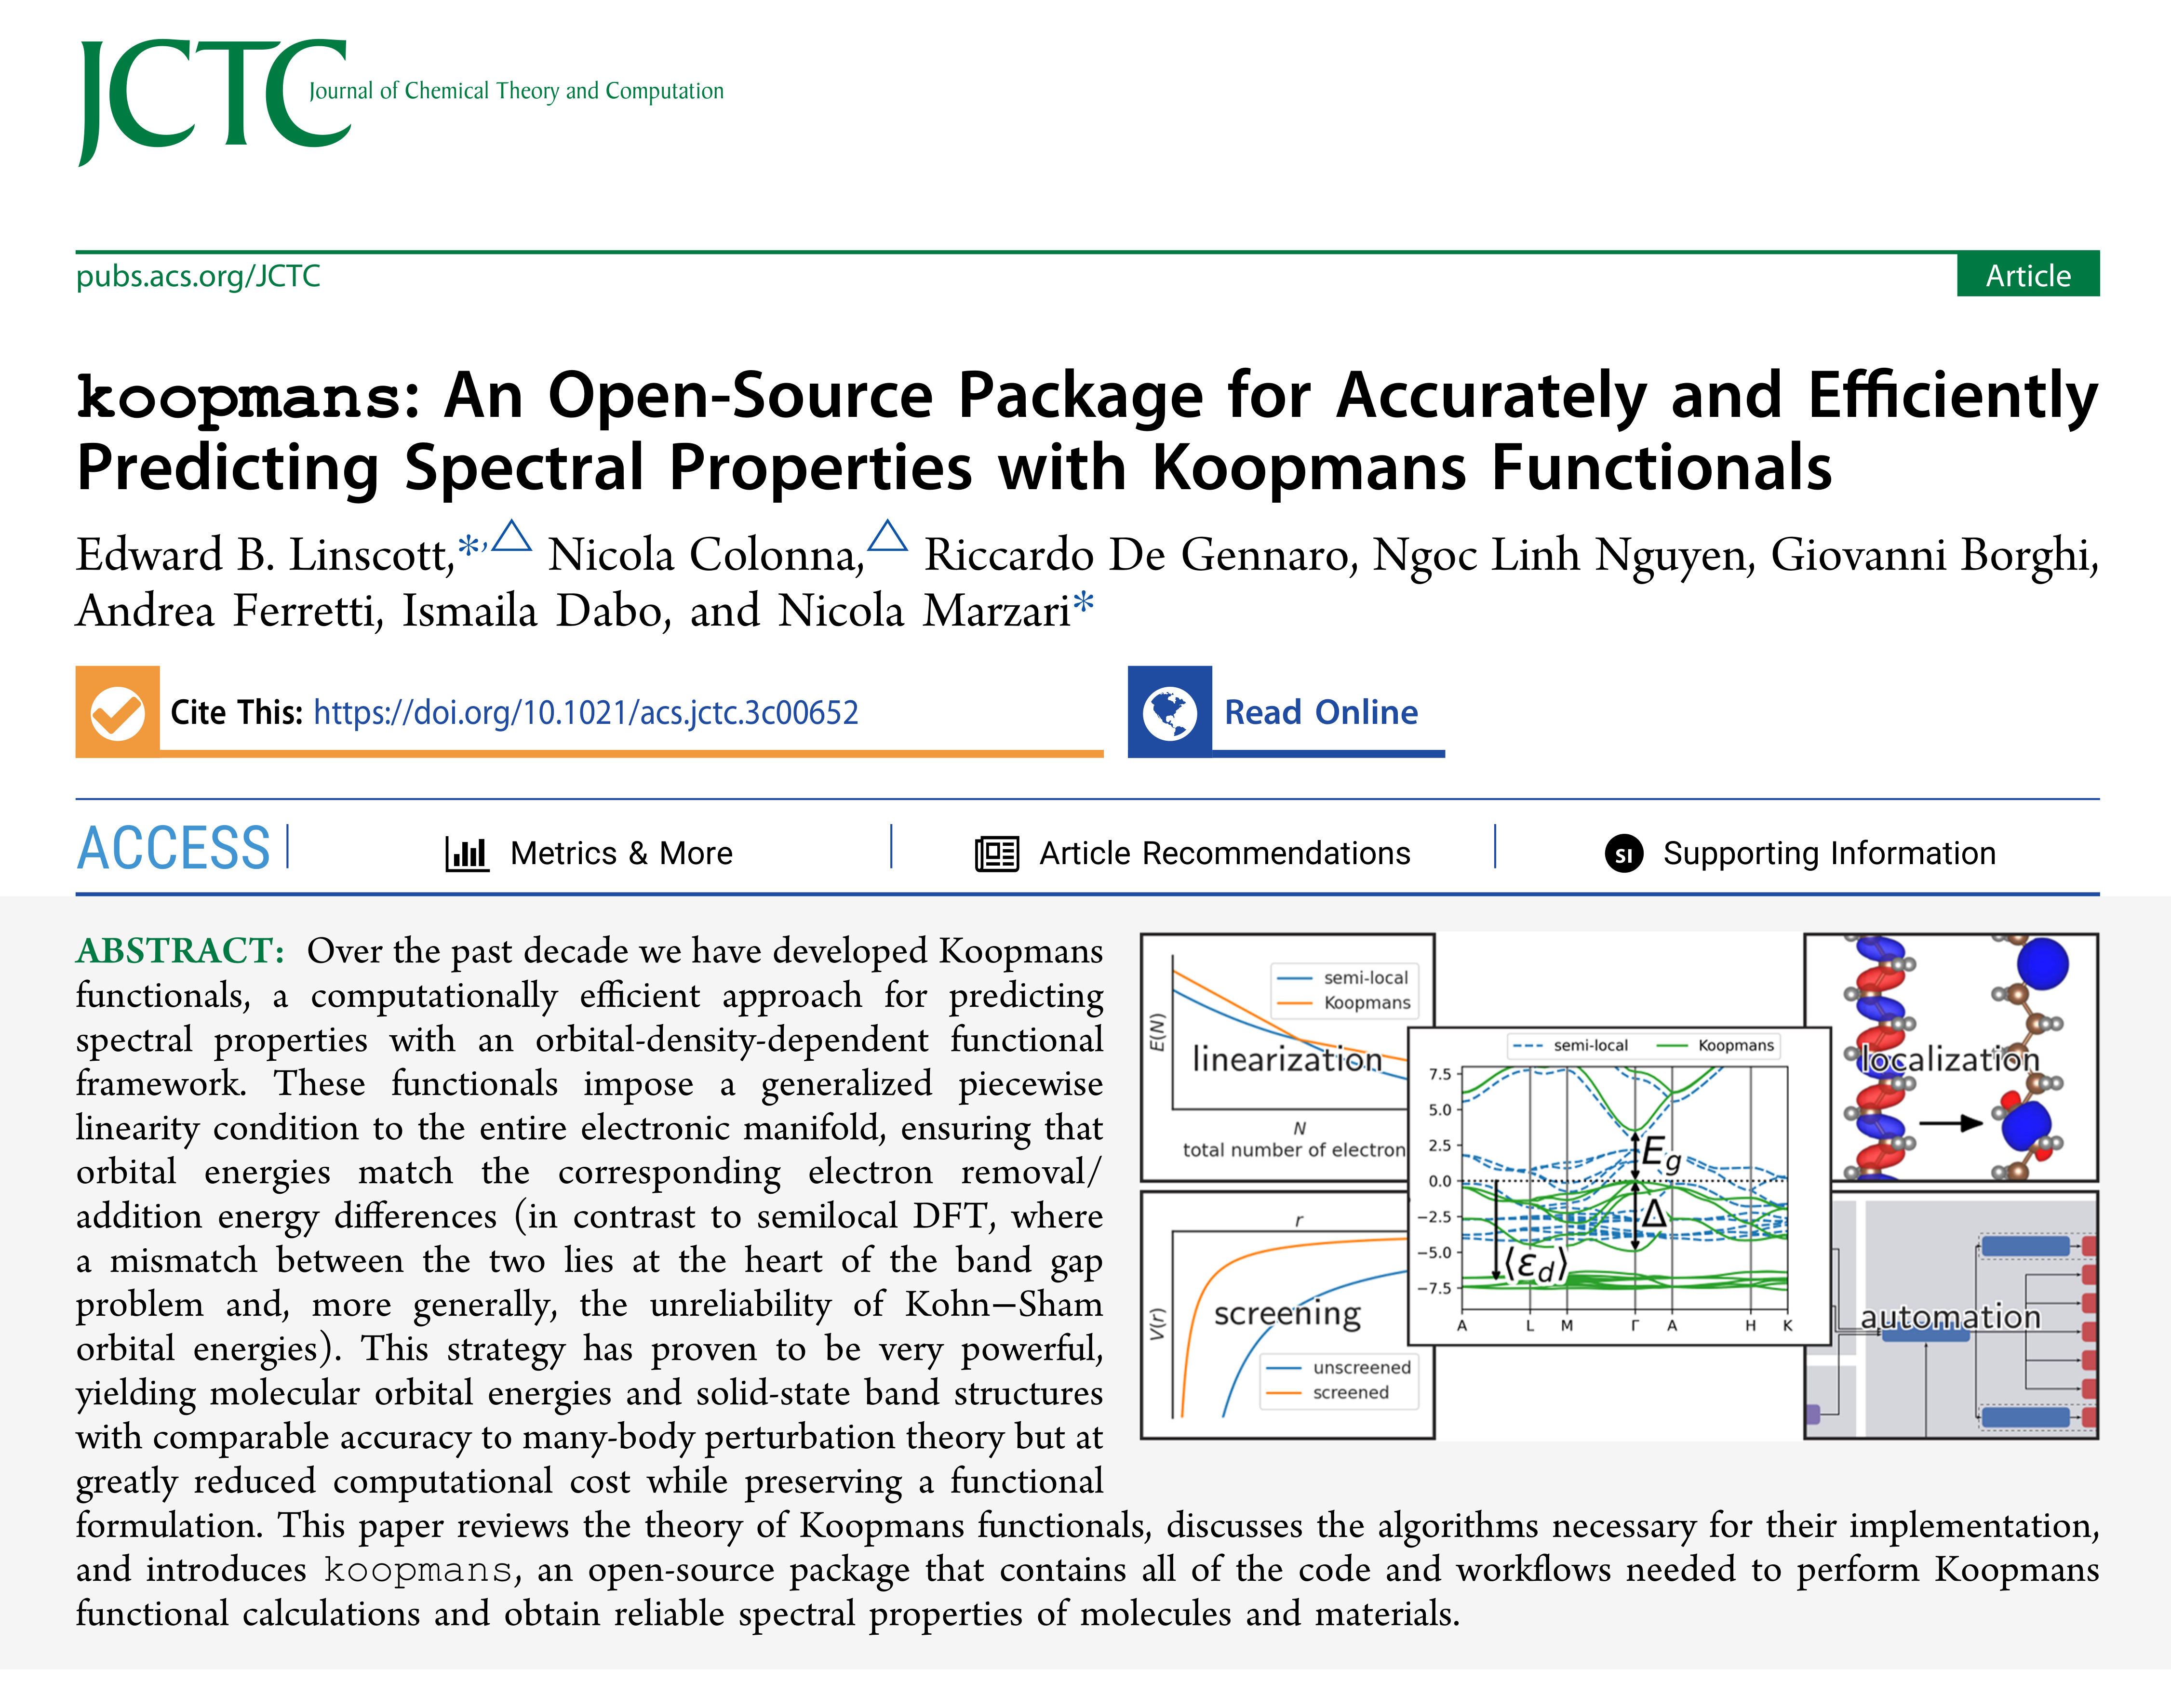
\includegraphics[width=\textwidth]{figures/jctc.png}
\end{frame}

\begin{frame}{Acknowledgements}

   \begin{center}
      \footnotesize
      \begin{tabularx}{\textwidth}{CCCC}
         \includegraphics[height = 0.3\paperheight]{figures/nicola_marzari.jpg}     &
         \includegraphics[height = 0.3\paperheight]{figures/nicola_colonna2.png}    &
         \includegraphics[height = 0.3\paperheight]{figures/riccardo_degennaro.jpg} &
         \includegraphics[height = 0.3\paperheight]{figures/yannick_schubert.jpg}     \\
         % \includegraphics[height = 0.2\paperheight]{figures/daniel_cole.jpeg}       &
         % \includegraphics[height = 0.2\paperheight]{figures/mike_payne.jpeg}        &
         % \includegraphics[height = 0.2\paperheight]{figures/david_oregan.jpg}         \\
         Nicola Marzari                                                             &
         Nicola Colonna                                                             &
         Riccardo De~Gennaro                                                        &
         Yannick Schubert                                                             \\
      \end{tabularx}
   \end{center}
   \begin{center}
      \includegraphics[height = 0.125\paperheight]{logos/SNF_logo_standard_print_color_pos_e.eps}
      \hspace{1em}
      \includegraphics[height = 0.15\paperheight]{figures/marvel_trimmed.png}
   \end{center}

   \vspace{1ex}
   \begin{center}
      Want to find out more? Go to \url{koopmans-functionals.org}
      \vspace{1em}
      Follow \includegraphics[height=\fontcharht\font`\B]{figures/Twitter_Bird.png} \textcolor{twitter_blue}{@ed\_linscott} for updates | Slides available at \includegraphics[height=\fontcharht\font`\B]{logos/github-favicon.png} github/elinscott
   \end{center}


   % \begin{multicols}{2}
   %    \tiny
   %    \printbibliography
   %    \normalsize
   % \end{multicols}
   \vspace{2ex}
   \scriptsize

   \setbeamercolor*{bibliography entry title}{fg=black}
   \setbeamercolor*{bibliography entry author}{fg=black}
   \setbeamercolor*{bibliography entry location}{fg=black}
   \setbeamercolor*{bibliography entry note}{fg=black}

   \vspace{2ex}
   \scriptsize
\end{frame}

\backupbegin
\begin{frame}{}

   \begin{center}
      \huge SPARE SLIDES
   \end{center}

\end{frame}

\begin{frame}{Koopmans functionals: off-diagonal occupancies}
   \begin{block}{Recap from earlier}
      Key idea: construct a functional such that the \emph{variational} orbital energies
      \begin{equation*}
         \varepsilon^\mathsf{Koopmans}_i = \braopket{\varphi_i}{H}{\varphi_i} = \partial E_\mathsf{Koopmans}/\partial f_i
      \end{equation*}
      are...
      \begin{itemize}
         \item independent of the corresponding occupancies $f_i$
         \item equal to the corresponding total energy difference $E_i(N-1) - E(N)$
      \end{itemize}
   \end{block}

   zero band gap $\rightarrow$ occupancy matrix for variational orbitals is off-diagonal
\end{frame}


% \begin{frame}{References}
%    \setbeamercolor*{bibliography entry title}{fg=black}
%    \setbeamercolor*{bibliography entry author}{fg=black}
%    \setbeamercolor*{bibliography entry location}{fg=black}
%    \setbeamercolor*{bibliography entry note}{fg=black}
%    \printbibliography
%    % For further reading on Koopmans functionals, see \cite{Dabo2010,Borghi2014,Nguyen2018,Colonna2018,Colonna2019,DeGennaro2022,Colonna2022}
% 
% \end{frame}
\begin{frame}{Learning the screening parameters}
   \begin{center}
      \begin{tikzpicture}
         \node[inner sep=0pt] (water box) at (0,0)
         {
            \includegraphics[width=0.25\textwidth]{figures/orbital.emp.00191_cropped.png}
         };
         \node[below=0cm of water box] (density) {$\rho_i(\mathbf{r})$};
         \node[right=0.2\textwidth of water box] (power spectrum) {
            $
               \begin{bmatrix}
                  x_{0} \\
                  x_{1} \\
                  x_{2} \\
                  \vdots
               \end{bmatrix}
            $
         };
         \path[line] (water box) -- node [midway, above, align=center] (decomposition) {power spectrum \\ decomposition} (power spectrum);
         \node[right=0.2\textwidth of power spectrum] (screening parameter) {$\alpha_i$};
         \path[line] (power spectrum) -- node [midway, above, align=center] (model) {ML model} (screening parameter);
      \end{tikzpicture}
   \end{center}

   \vspace{-4em}

   \blfootcite{Schubert2022}

   \begin{align*}
      c^i_{nlm,k=\mathsf{orbital}} & =\int d\textbf{r} g_{nl}(r)Y_{lm}(\theta,\varphi)\rho^i(\textbf{r}-\textbf{R}^i)                        \\
      p^i_{n_1n_2l,k_1k_2}         & =\pi \sqrt{\frac{8}{2l+1}}\sum\limits_m {c_{n_1lm,k_1}^{i *}}c_{n_2lm,k_2}^i \label{eq: power spectrum}
   \end{align*}

   % $g_{nl}$ = orthonormalised radial Gaussian basis functions

   % $Y_{lm}$ = spherical harmonics

\end{frame}

\begin{frame}{Learning the screening parameters}
   \begin{center}

      \includegraphics[height=0.7\paperheight]{figures/CsSnI3_calc_vs_pred_Edward.png}
      \includegraphics[height=0.7\paperheight]{figures/convergence_analysis_Edward.png}

      loss of accuracy of the band gap of $\sim$ 0.02 eV

      (cf. when calculating screening parameters \emph{ab initio})

      speedup of 70$\times$
   \end{center}

   \blfootcite{Schubert2022}

\end{frame}

\begin{frame}{Resonance with other efforts}
   \begin{itemize}
      \item Wannier transition-state method of Anisimov and Kozhevnikov \cite{Anisimov2005}
      \item Optimally tuned hybrid functionals of Kronik, Pasquarello, and others (refer back to Leeor's talk on Wednesday) \cite{Kronik2012,Wing2021}
      \item Ensemble DFT of Kronik and co-workers \cite{Kraisler2013}
      \item Koopmans-Wannier of Wang and co-workers \cite{Ma2016}
      \item Dielectric-dependent hybrid functionals of Galli and co-workers \cite{Skone2016a}
      \item LOSC functionals of Yang and co-workers \cite{Li2018}
   \end{itemize}
\end{frame}




\backupend
\end{document}
